%% Beispiel-Präsentation mit LaTeX Beamer im KIT-Design
%% entsprechend den Gestaltungsrichtlinien vom 1. August 2020
%%
%% Siehe https://sdqweb.ipd.kit.edu/wiki/Dokumentvorlagen

%% Beispiel-Präsentation
\documentclass[en]{sdqbeamer} 
 
%% Titelbild
\titleimage{../images/title_header_5}

%% Gruppenlogo
\grouplogo{teco_logo.png} 

%% Gruppenname und Breite (Standard: 50 mm)
\groupname{
Chair of Pervasive Computing Systems/TECO\\
Institute of Telematics, Department of Informatics\\
}
%\groupnamewidth{50mm}

% Beginn der Präsentation

\title[Ear-Based Temperature Probing]{Ear-Based Temperature Probing: \\ Sensor Placement and Fusion for Wearable Applications}
\subtitle{Chair of Pervasive Computing Systems / TECO} 
\author[David Laubenstein]{David Laubenstein, Supervisor: Tobias Röddiger}

\date[11/08/2023]{Nov 08, 2023}

% Literatur 
 
\usepackage[bibstyle=numeric,hyperref,backend=biber]{biblatex}
\usepackage[inkscapeformat=png]{svg}
\usepackage{tabularx}
\addbibresource{../thesis-doc/Literature.bib}
\bibhang1em

\begin{document}
 
%Titelseite
\KITtitleframe

%Inhaltsverzeichnis
% sollte weg laut betreuern
% \begin{frame}{Inhaltsverzeichnis}
% \tableofcontents
% \end{frame}

\section{Motivation}
\begin{frame}{Motivation}
    \begin{itemize}
        \item Current state of temperature measurement \cite{TemperatureDigitalGlassa}
        \item No long-term measurement possible
    \end{itemize}
    \begin{center}
        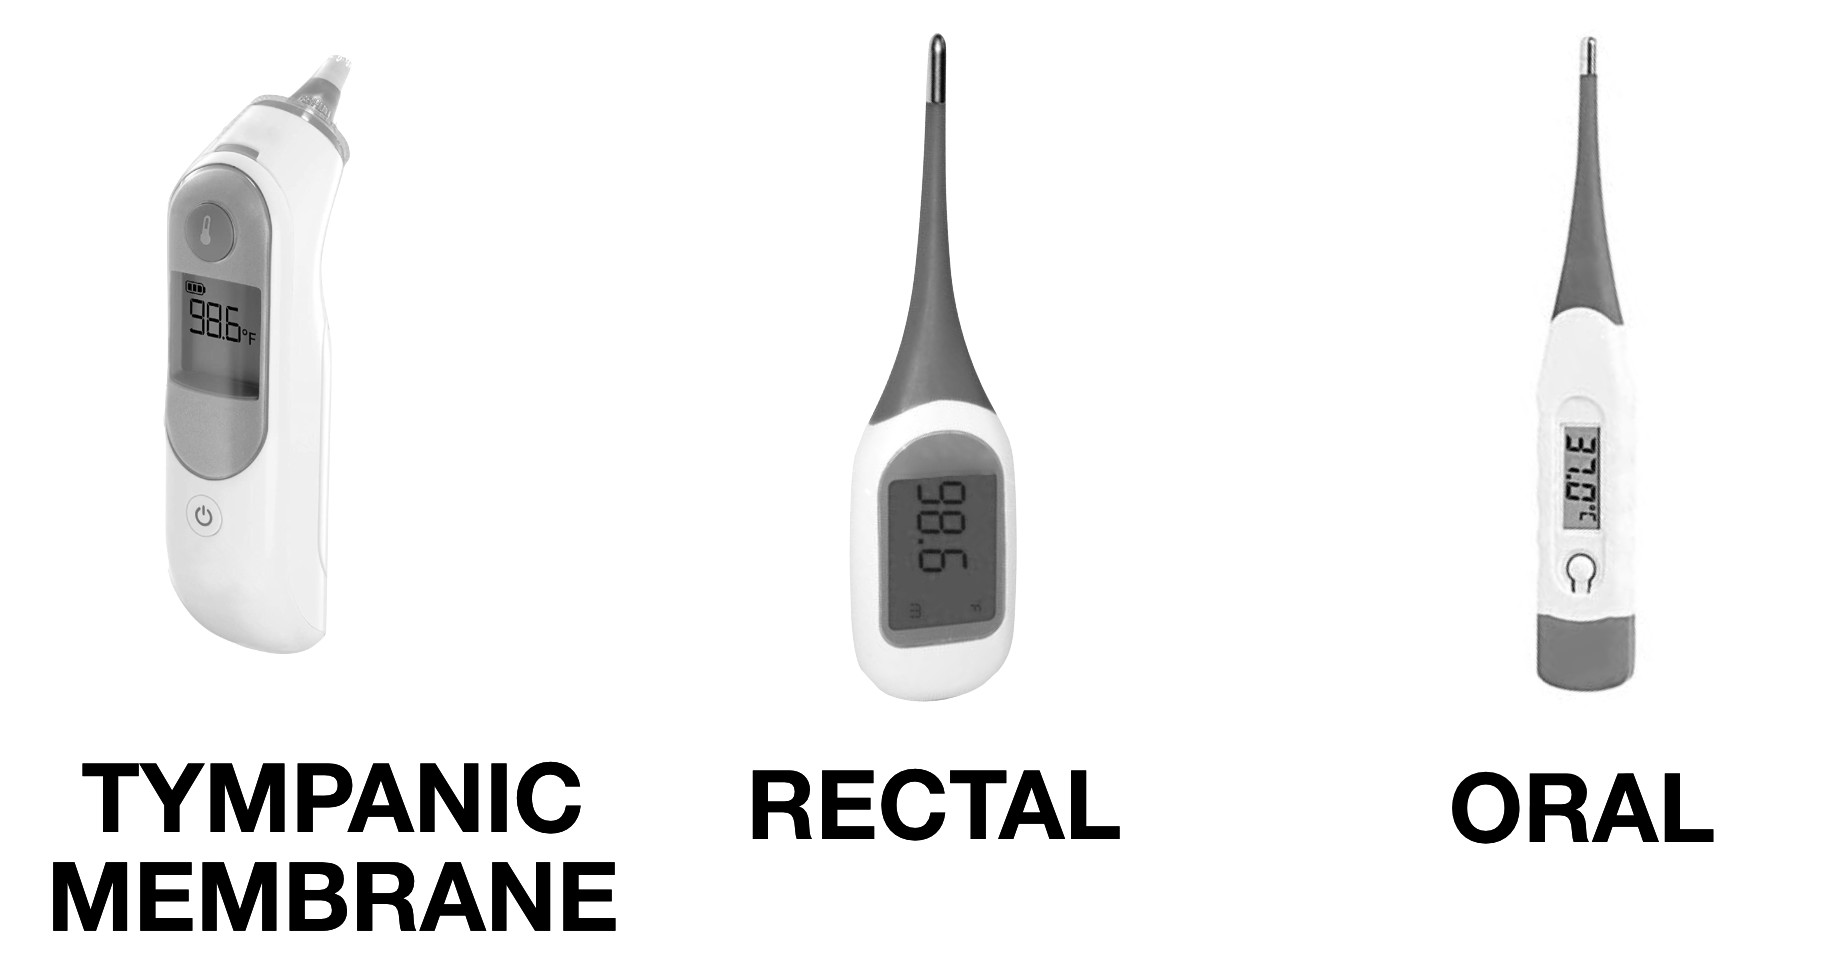
\includegraphics[scale=0.15]{proposal-presentation/images/thermometer_types.jpg}    
    \end{center}
\end{frame}

\begin{frame}{Motivation}
    \begin{itemize}
        \item Solution: integration in wearables we already use a lot
    \end{itemize}
    \begin{center}
        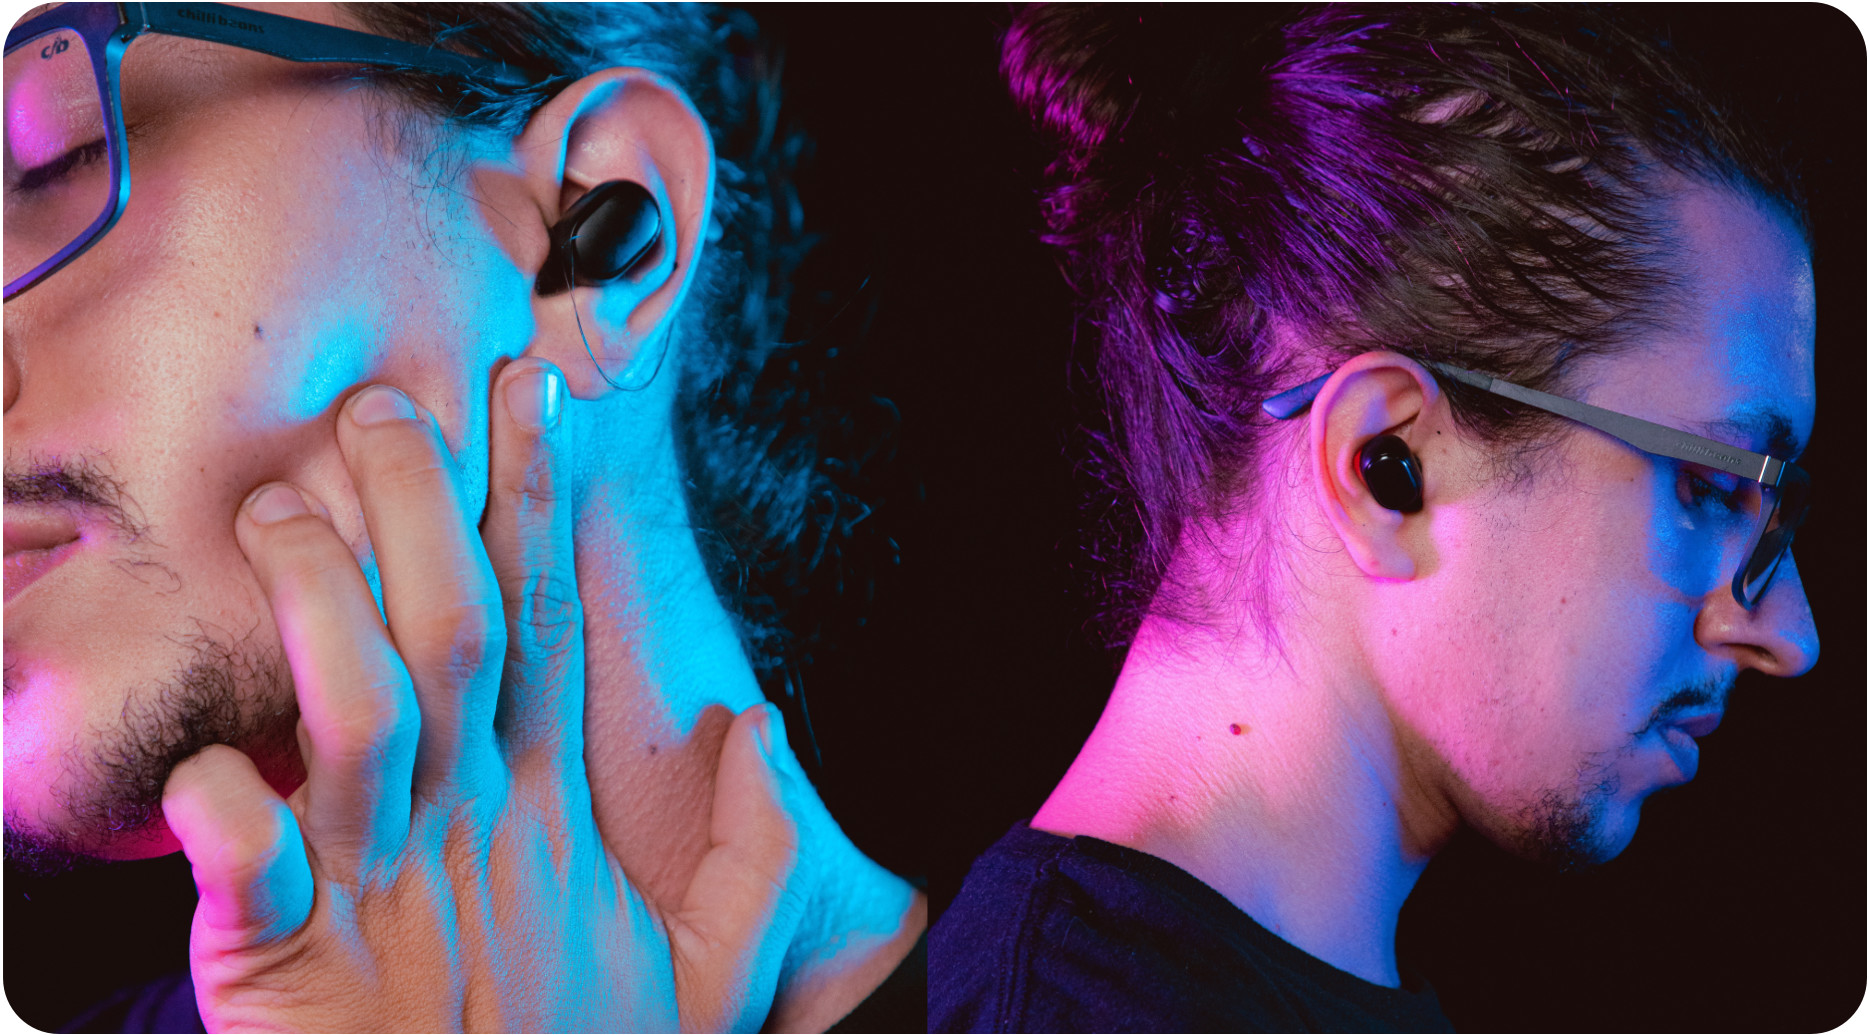
\includegraphics[scale=0.14]{proposal-presentation/images/inears/earbuds_picture.jpg}
    \end{center}
\end{frame}

% \section{Problem}
% \begin{frame}{Problem}
%     \begin{itemize}
%         \item accuracy and reliability
%         \begin{itemize}
%             \item sensor location
%             \item skin contact
%             \item calibration
%         \end{itemize}
%         \item tympanic membrane measurement set up
%         \begin{itemize}
%             \item alignment
%             \item ear wax
%         \end{itemize}
%     \end{itemize}
% \end{frame}

% \begin{frame}[fragile]{Question}
%     \begin{column}{0.50\textwidth}
%         \begin{itemize}
%             \item measures temperature at different locations in and around the ears
%             \item hypotheses
%             \begin{itemize}
%                 \item correlations with activity
%                 \item quality can be improved through IMU
%                 \item combination of signals improves the quality
%                 \item Skin temperature around the ear strongly correlates with core body temperature.
%             \end{itemize}
%         \end{itemize}
%     \end{column}
%     \begin{column}{0.45\textwidth}
%         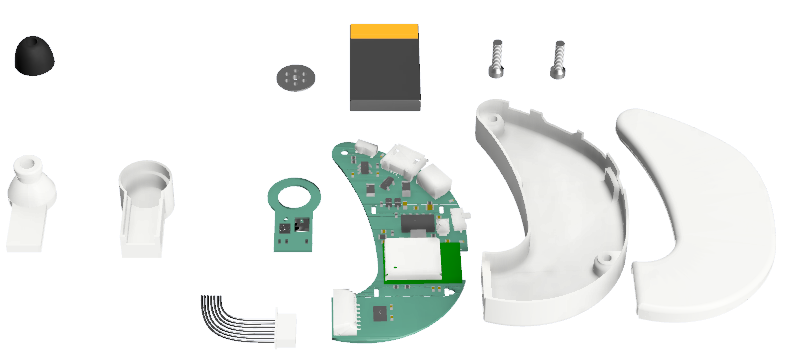
\includegraphics[scale=0.26]{proposal-presentation/images/open_earable_new.png}
%     \end{column}
% \end{frame}

% \begin{frame}[fragile]{Related Work}
% \begin{column}{0.47\textwidth}
%         \begin{itemize}
%         \item huge research field for ...
%         \begin{itemize}
%             \item temperature measurement on the tympanic membrane
%             \item body temperature measurement
%         \end{itemize}
%         \item no studies on other positions in/around the ear
%     \end{itemize}
%     \vspace{1cm}
%     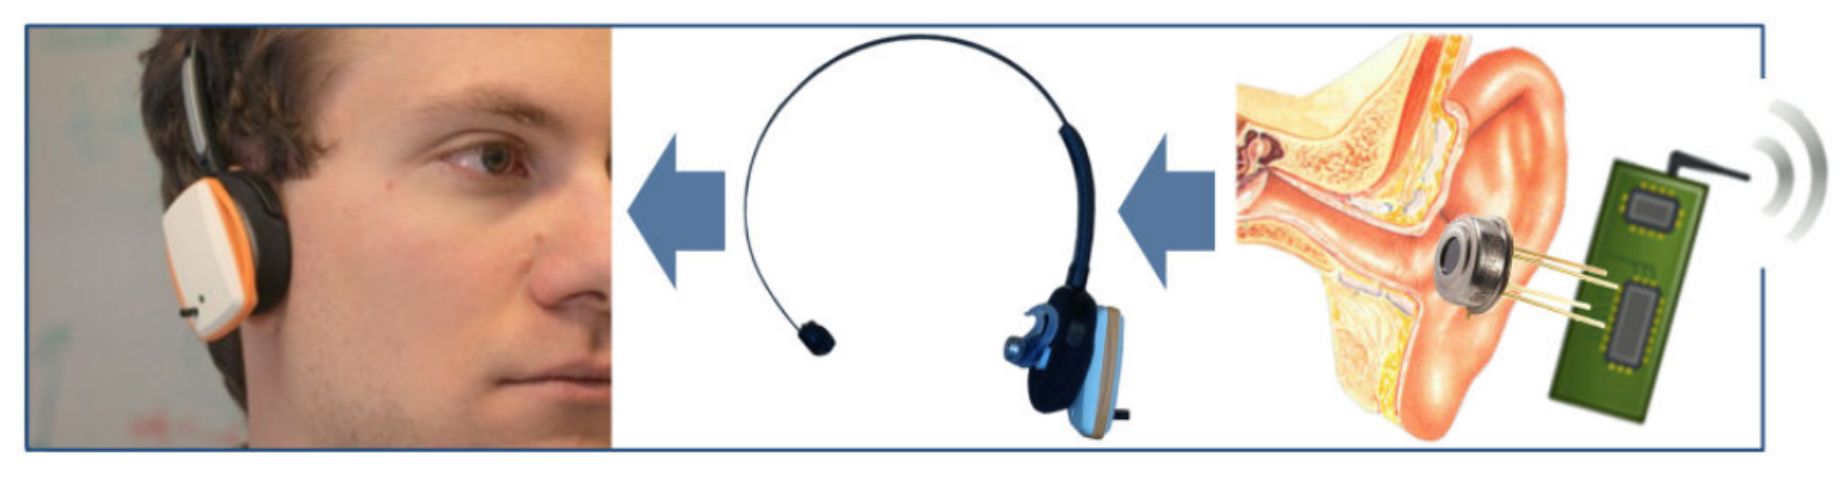
\includegraphics[scale=0.26]{proposal-presentation/images/relatedWork/relatedWork3.png}
%     \end{column}
%     \begin{column}{0.43\textwidth}
%     \vspace{-0.4cm}
%         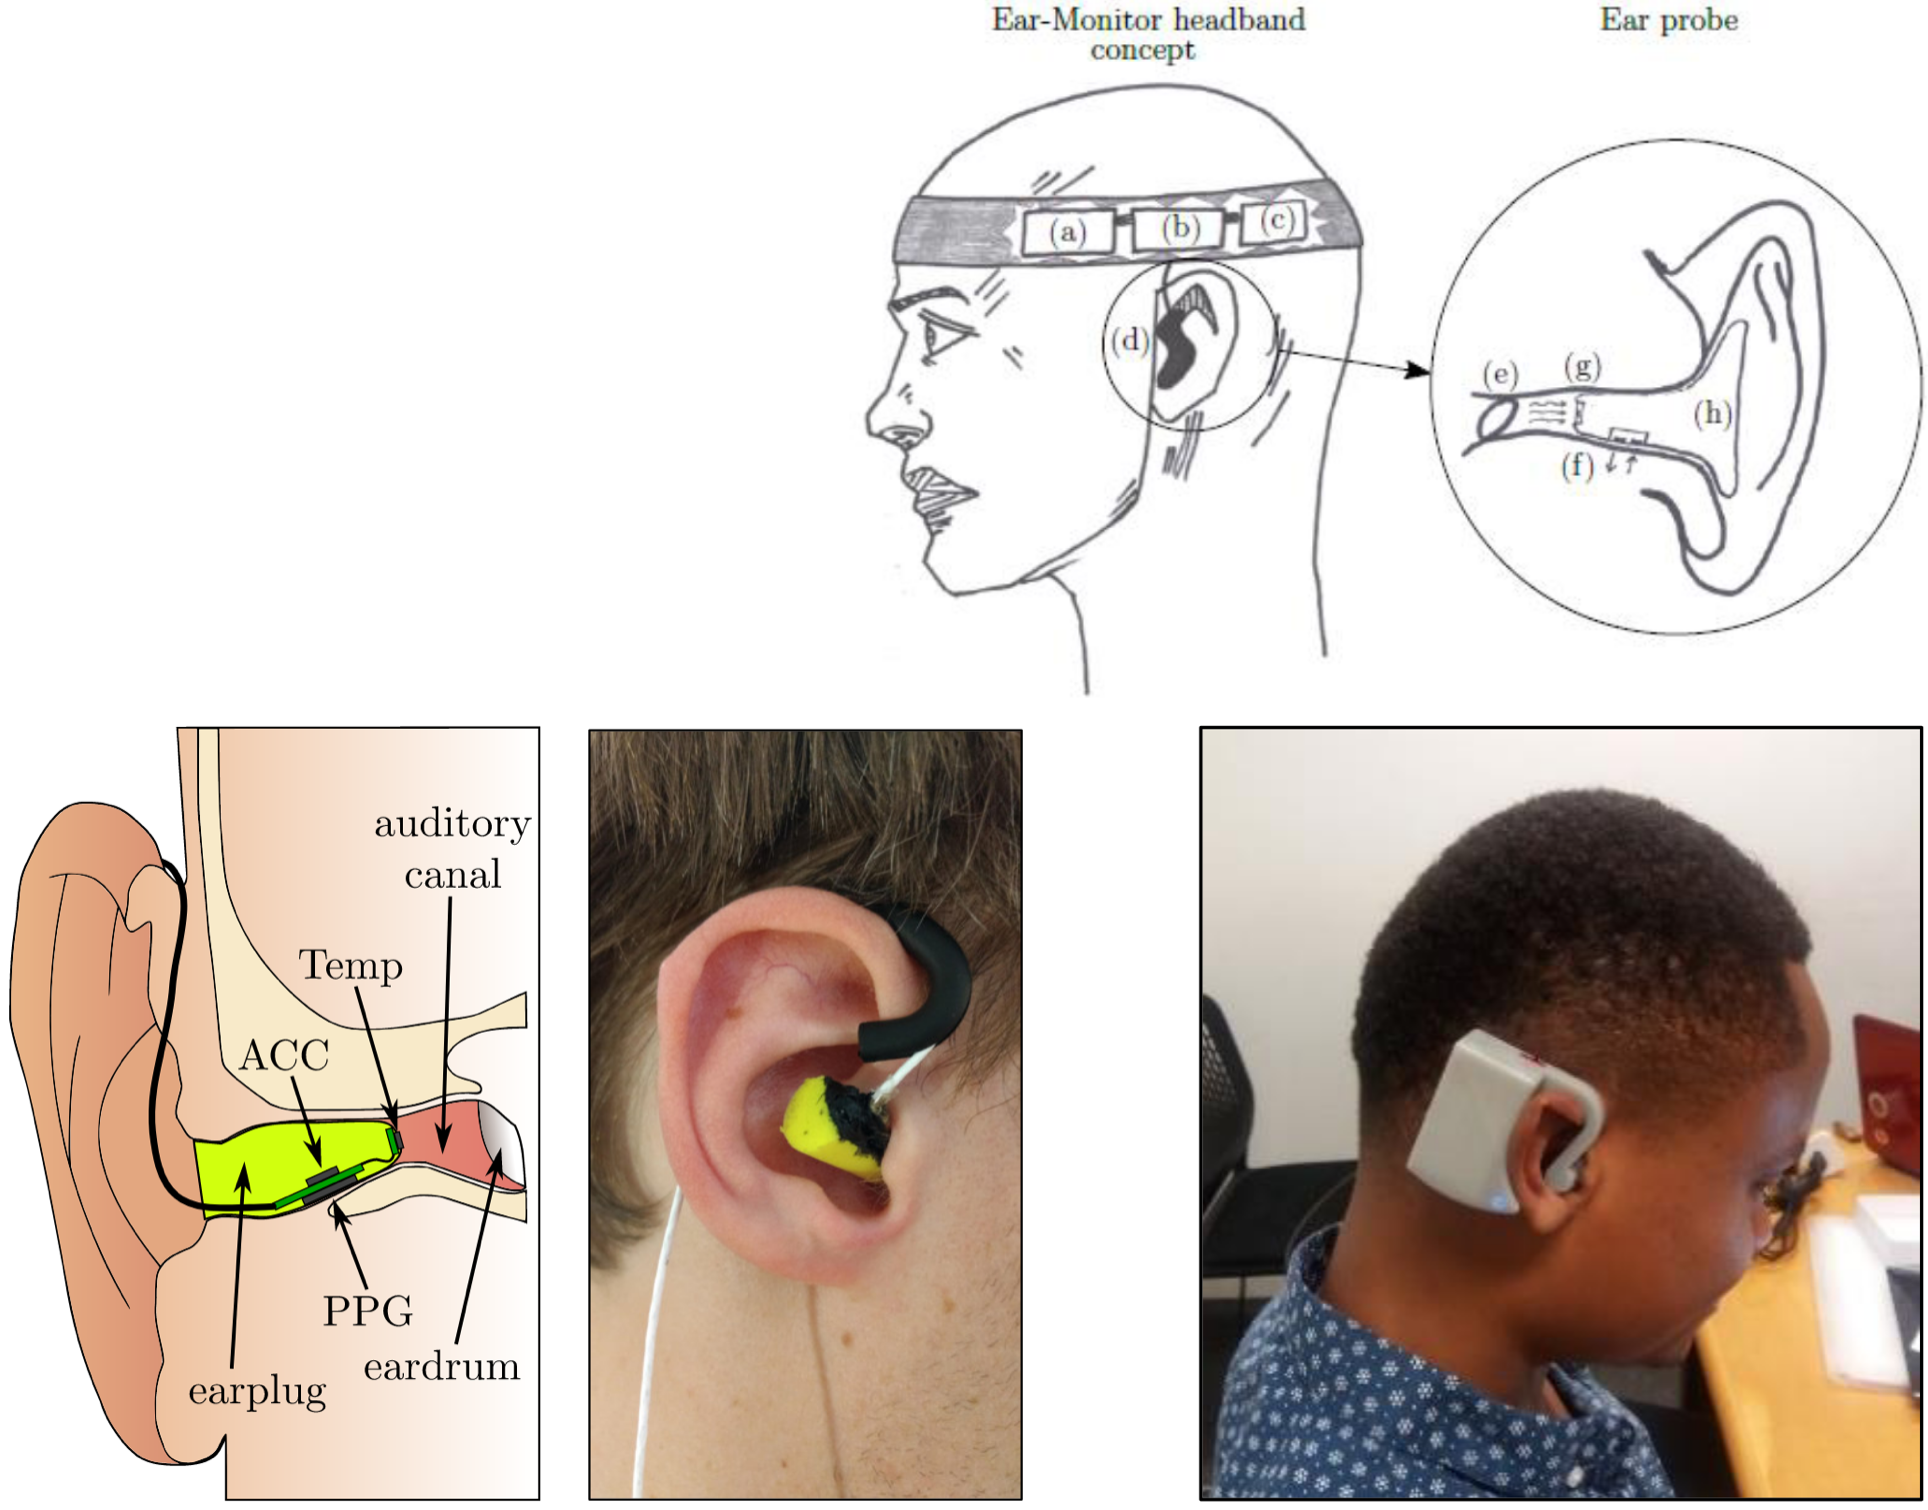
\includegraphics[scale=0.19]{proposal-presentation/images/relatedWork/relatedWorkMerged2.png}
%     \end{column}
% \end{frame}

\section{Planned Approach}
\begin{frame}{Planned Approach}
    \begin{itemize}
        \item Device to measure ear-based temperature data
        \begin{itemize}
            \item OpenEarable platform adaption
            \item MLX temperature sensor
        \end{itemize}
        \item 2 studies (baseline surveys and environmental influences, under stress conditions)
    \end{itemize}
    \begin{center}
        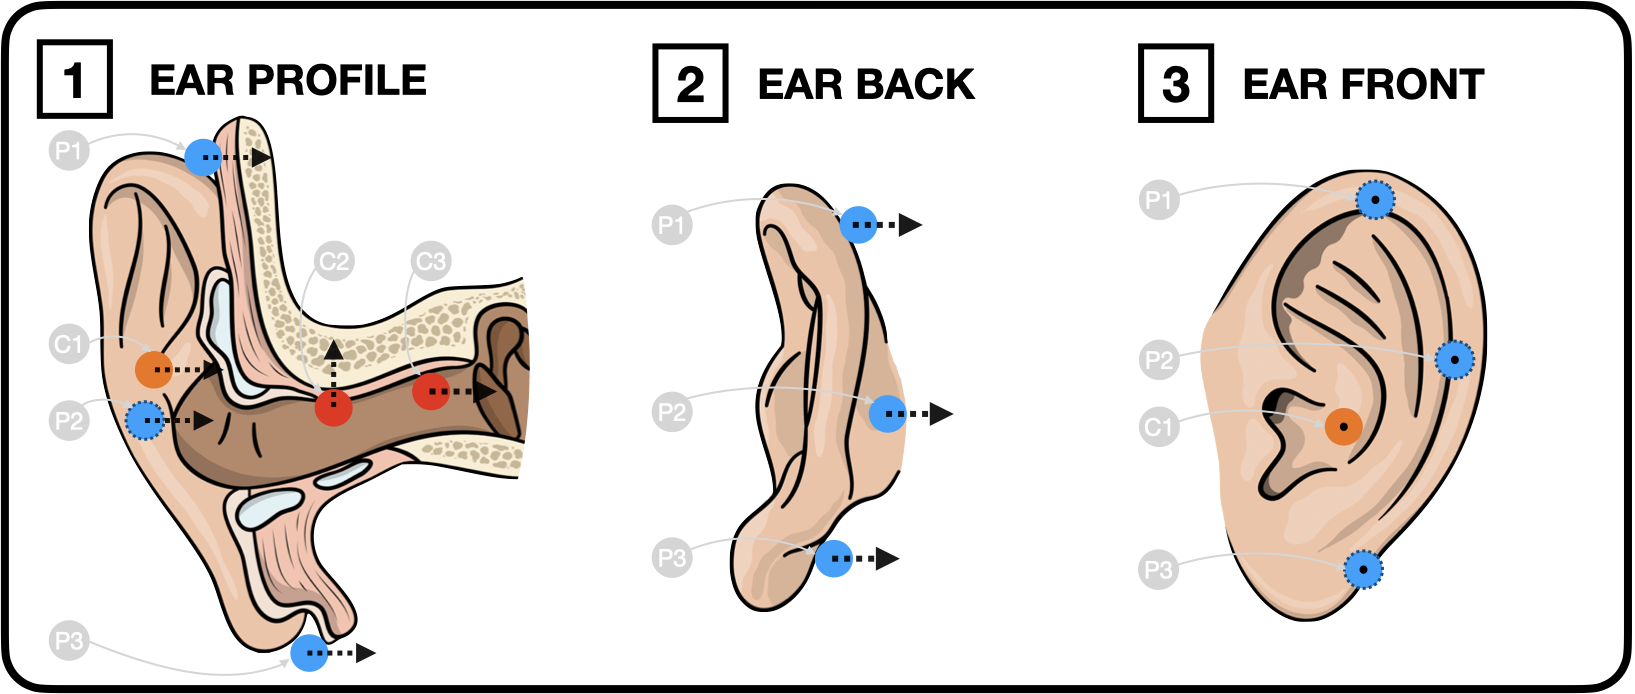
\includegraphics[scale=0.17]{../thesis-doc/images/ear_measurement_points/emp.png}    
    \end{center}
\end{frame}

% \section{Expected Result}
% \begin{frame}{Expected Result}
%     \begin{itemize}
%         \item insights into sensor placement in/around the ear
%         \item combination of sensors to improve data quality
%         \item supports the development of more accurate and reliable wearable devices for biometric applications
%     \end{itemize}
% \end{frame}

\section{Prototype}
\begin{frame}{Prototype}
    \begin{center}
      \begin{columns}[T]
        \begin{column}{.48\textwidth}
          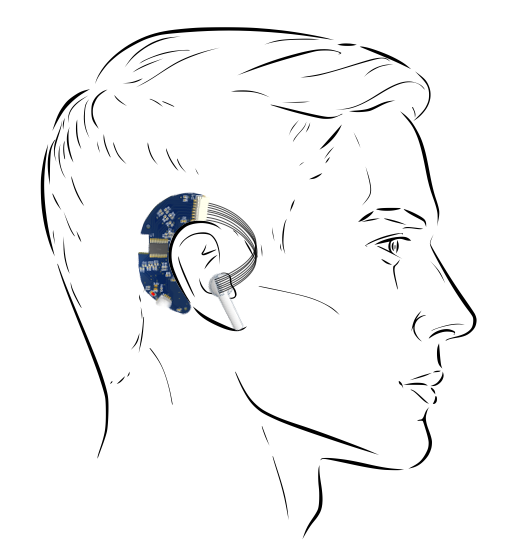
\includegraphics[width=0.7\linewidth]{../thesis-doc/images/prototype/prototype_on_head_visual.png}
        \end{column}
        
        \begin{column}{.48\textwidth}
          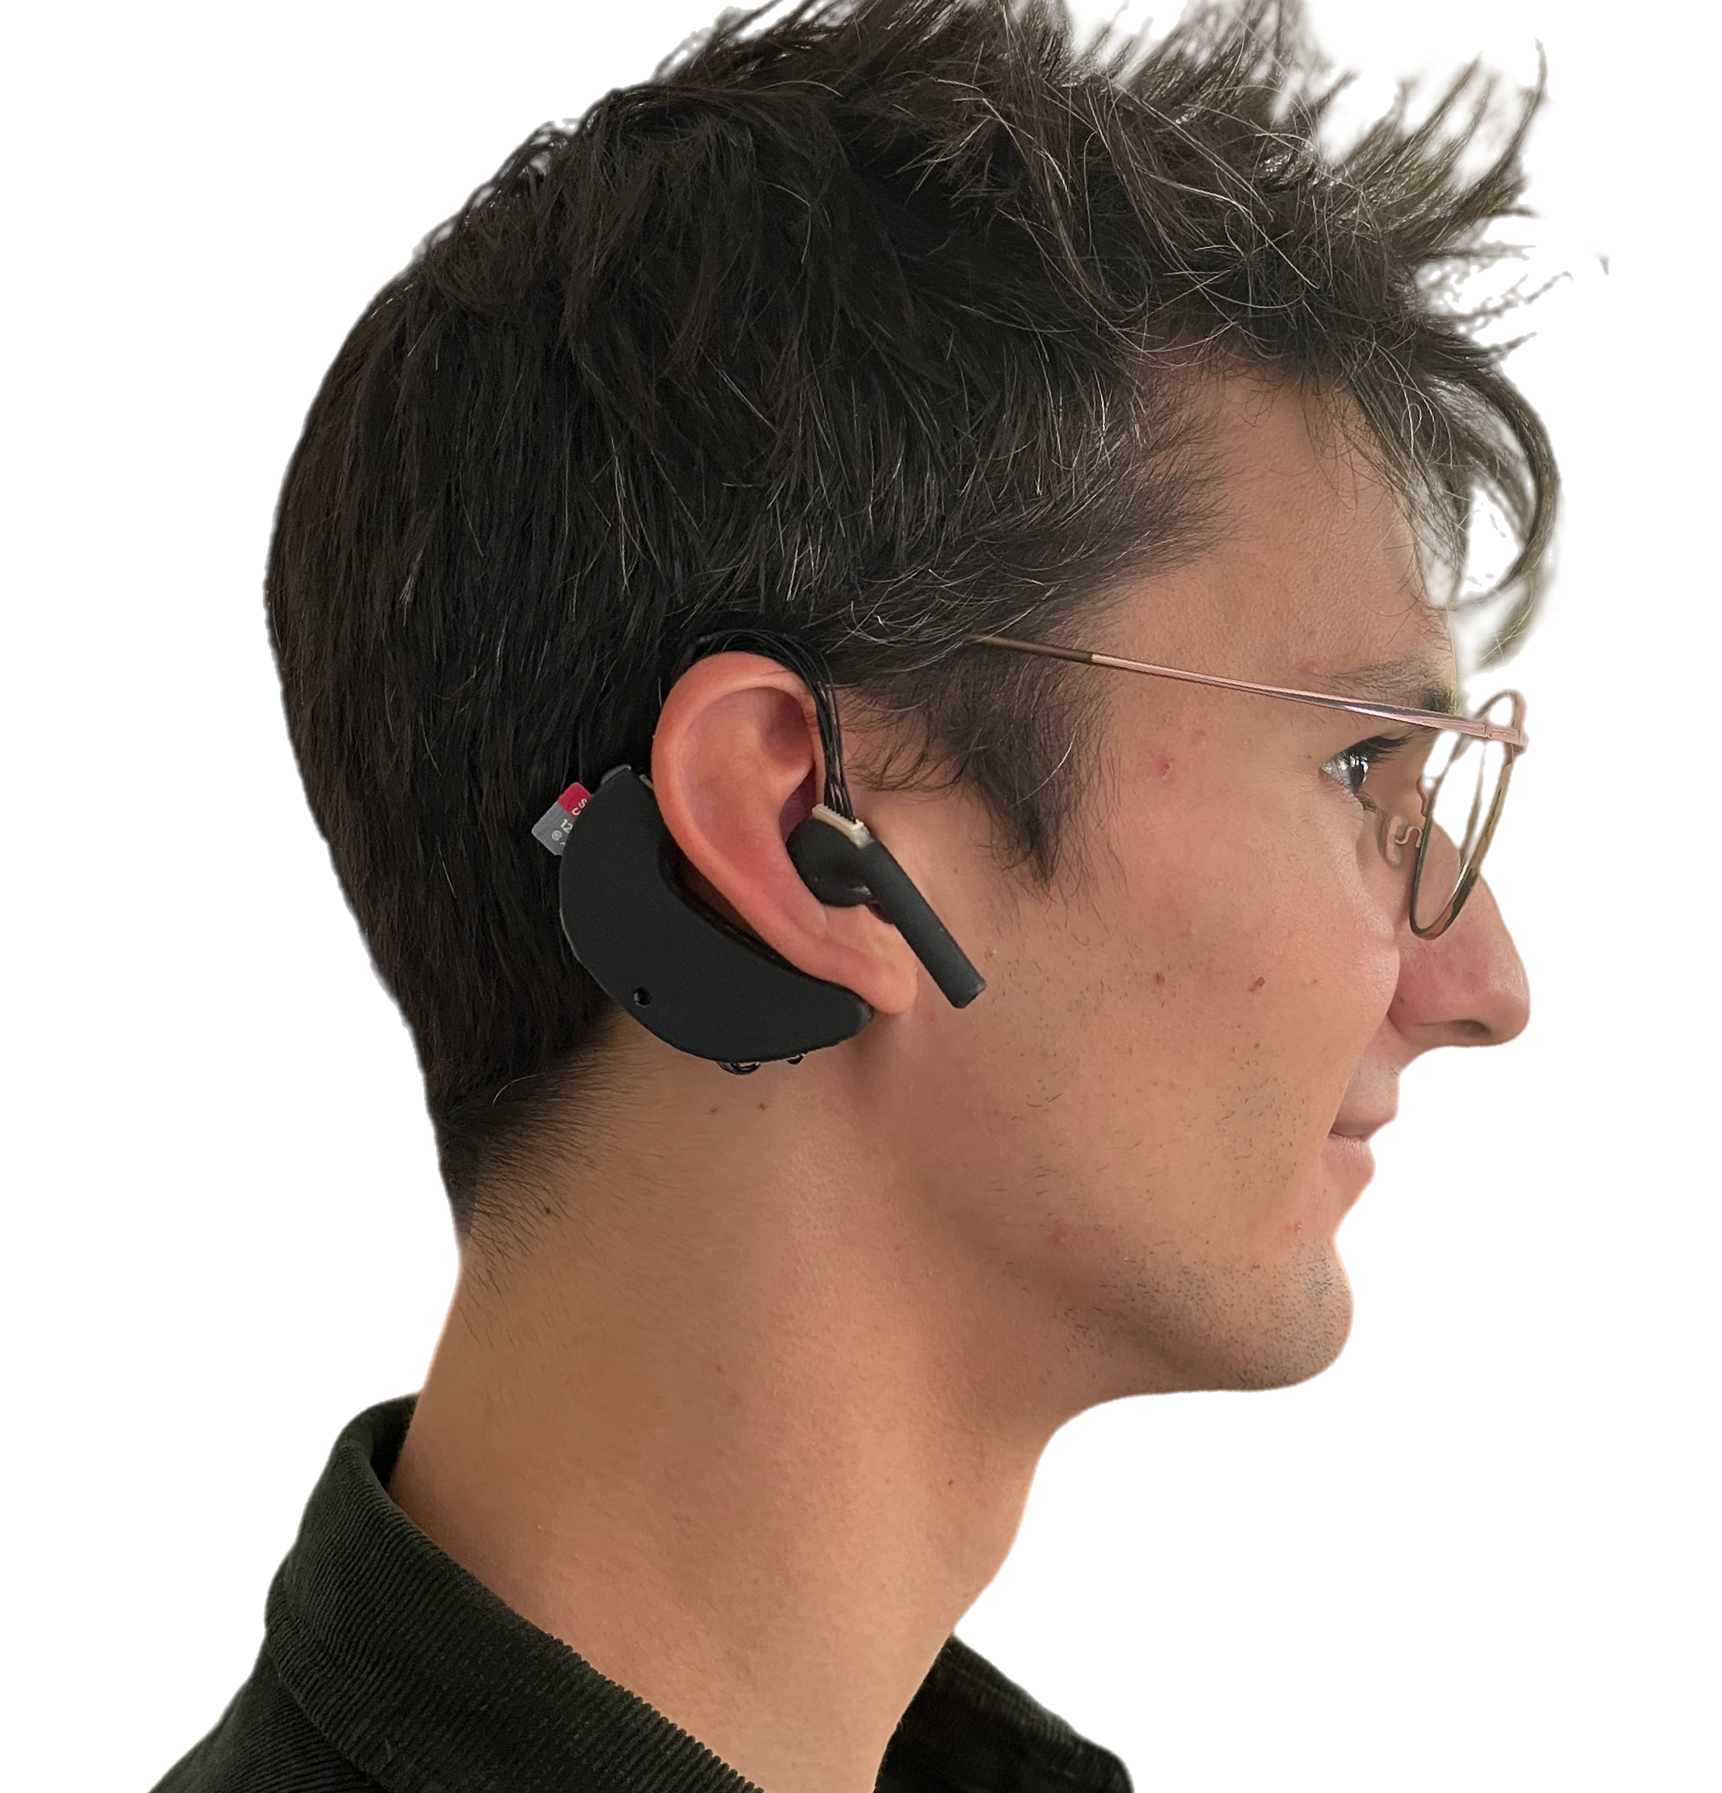
\includegraphics[width=0.75\linewidth]{../thesis-doc/images/prototype/Lorenz.png} 
        \end{column}
      \end{columns}
    \end{center}
\end{frame}

\begin{frame}{Prototype: Main Hardware Connection}
    \begin{columns}[T]
        \begin{column}{.34\textwidth}
          \begin{itemize}
              \item Communication between components with I2C
              \item OpenEarable
              \begin{itemize}
                  \item SD card
                  \item Arduino Nano 33 BLE
                  \item IMU
                  \item Status LED
                  \item Clicky button
              \end{itemize}
              \item PCB
              \item FlexPCB
          \end{itemize}
        \end{column}
        
        \begin{column}{.64\textwidth}
          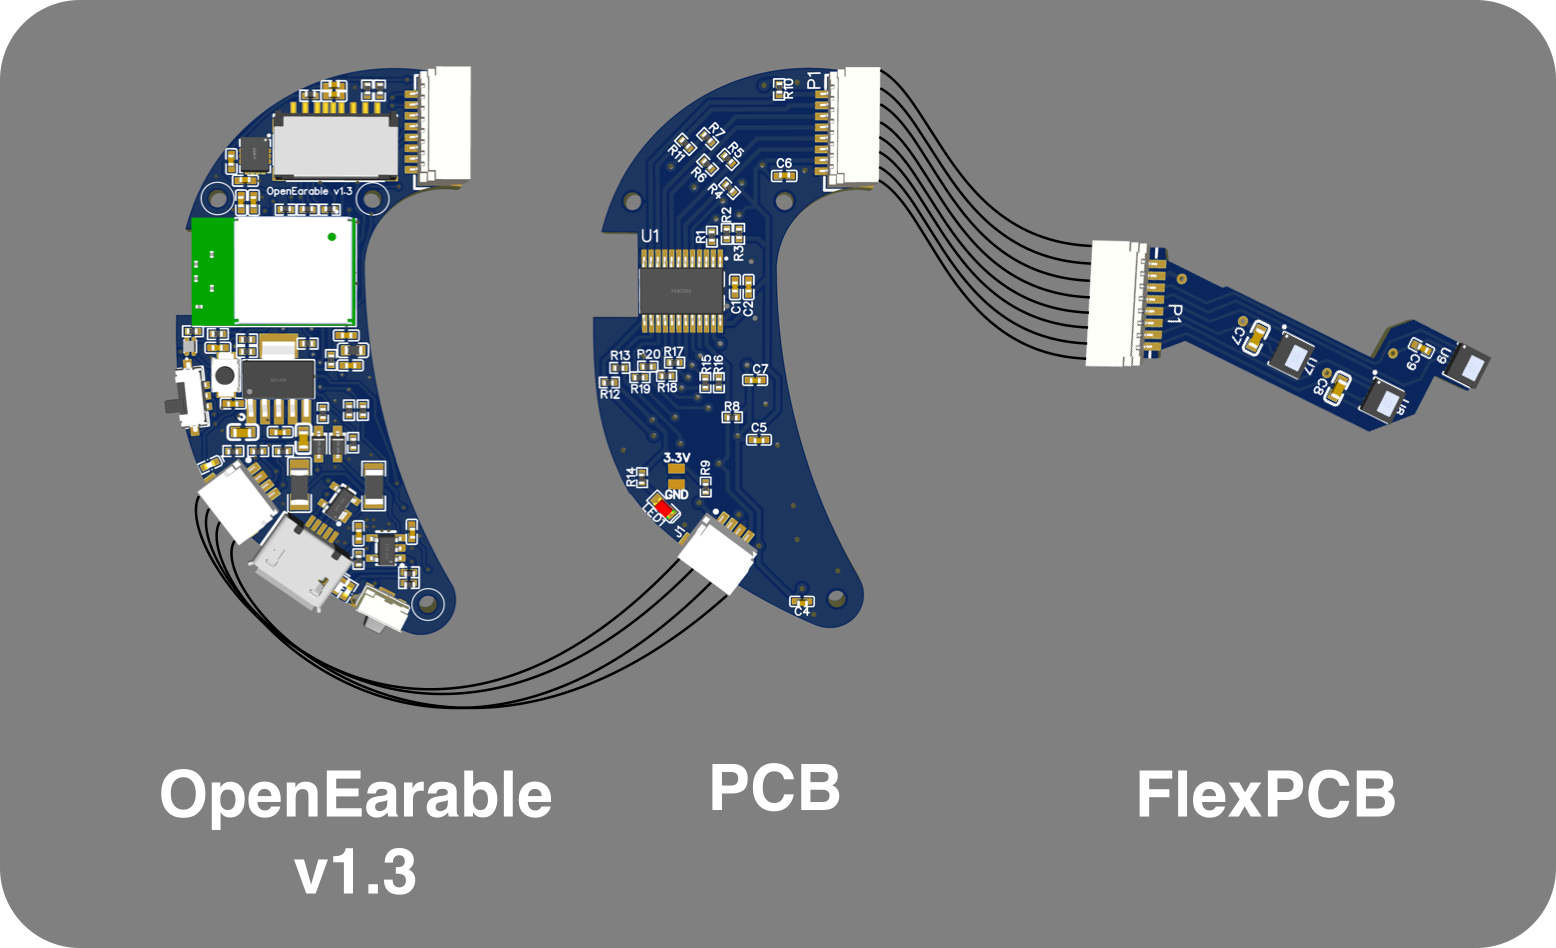
\includegraphics[width=0.95\linewidth]{../thesis-doc/images/prototype/PrototypeConnection.png}
        \end{column}
      \end{columns}
\end{frame}

\begin{frame}{Prototype: PCB Composition}
    \begin{columns}[T]
        \begin{column}{.34\textwidth}
          \begin{itemize}
              \item 4-pin and 8-pin connector to connect OpenEarable and FlexPCB
              \item Multiplexer
              \begin{itemize}
                  \item Switch through one of 8 channels
                  \item Each temperature sensor is connected
              \end{itemize}
              \item MLX90632 temperature sensor
              \begin{itemize}
                  \item Infrared sensor
                  \item Factory calibrated
                  \item Accuracy of $\pm0.2^\circ\text{C}$
              \end{itemize}
              \item LED
          \end{itemize}
        \end{column}
        
        \begin{column}{.64\textwidth}
          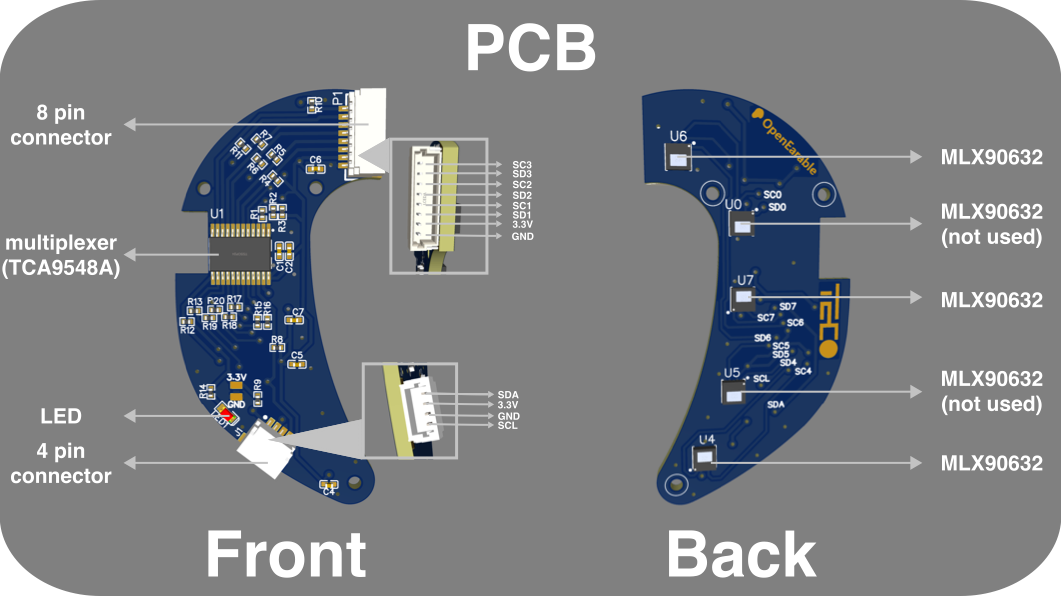
\includegraphics[width=0.95\linewidth]{../thesis-doc/images/prototype/PCB_Description.png}
        \end{column}
      \end{columns}
\end{frame}

\begin{frame}{Prototype: FlexPCB - Concept vs Final Design}
\begin{columns}[T]
    \begin{column}{.48\textwidth}
      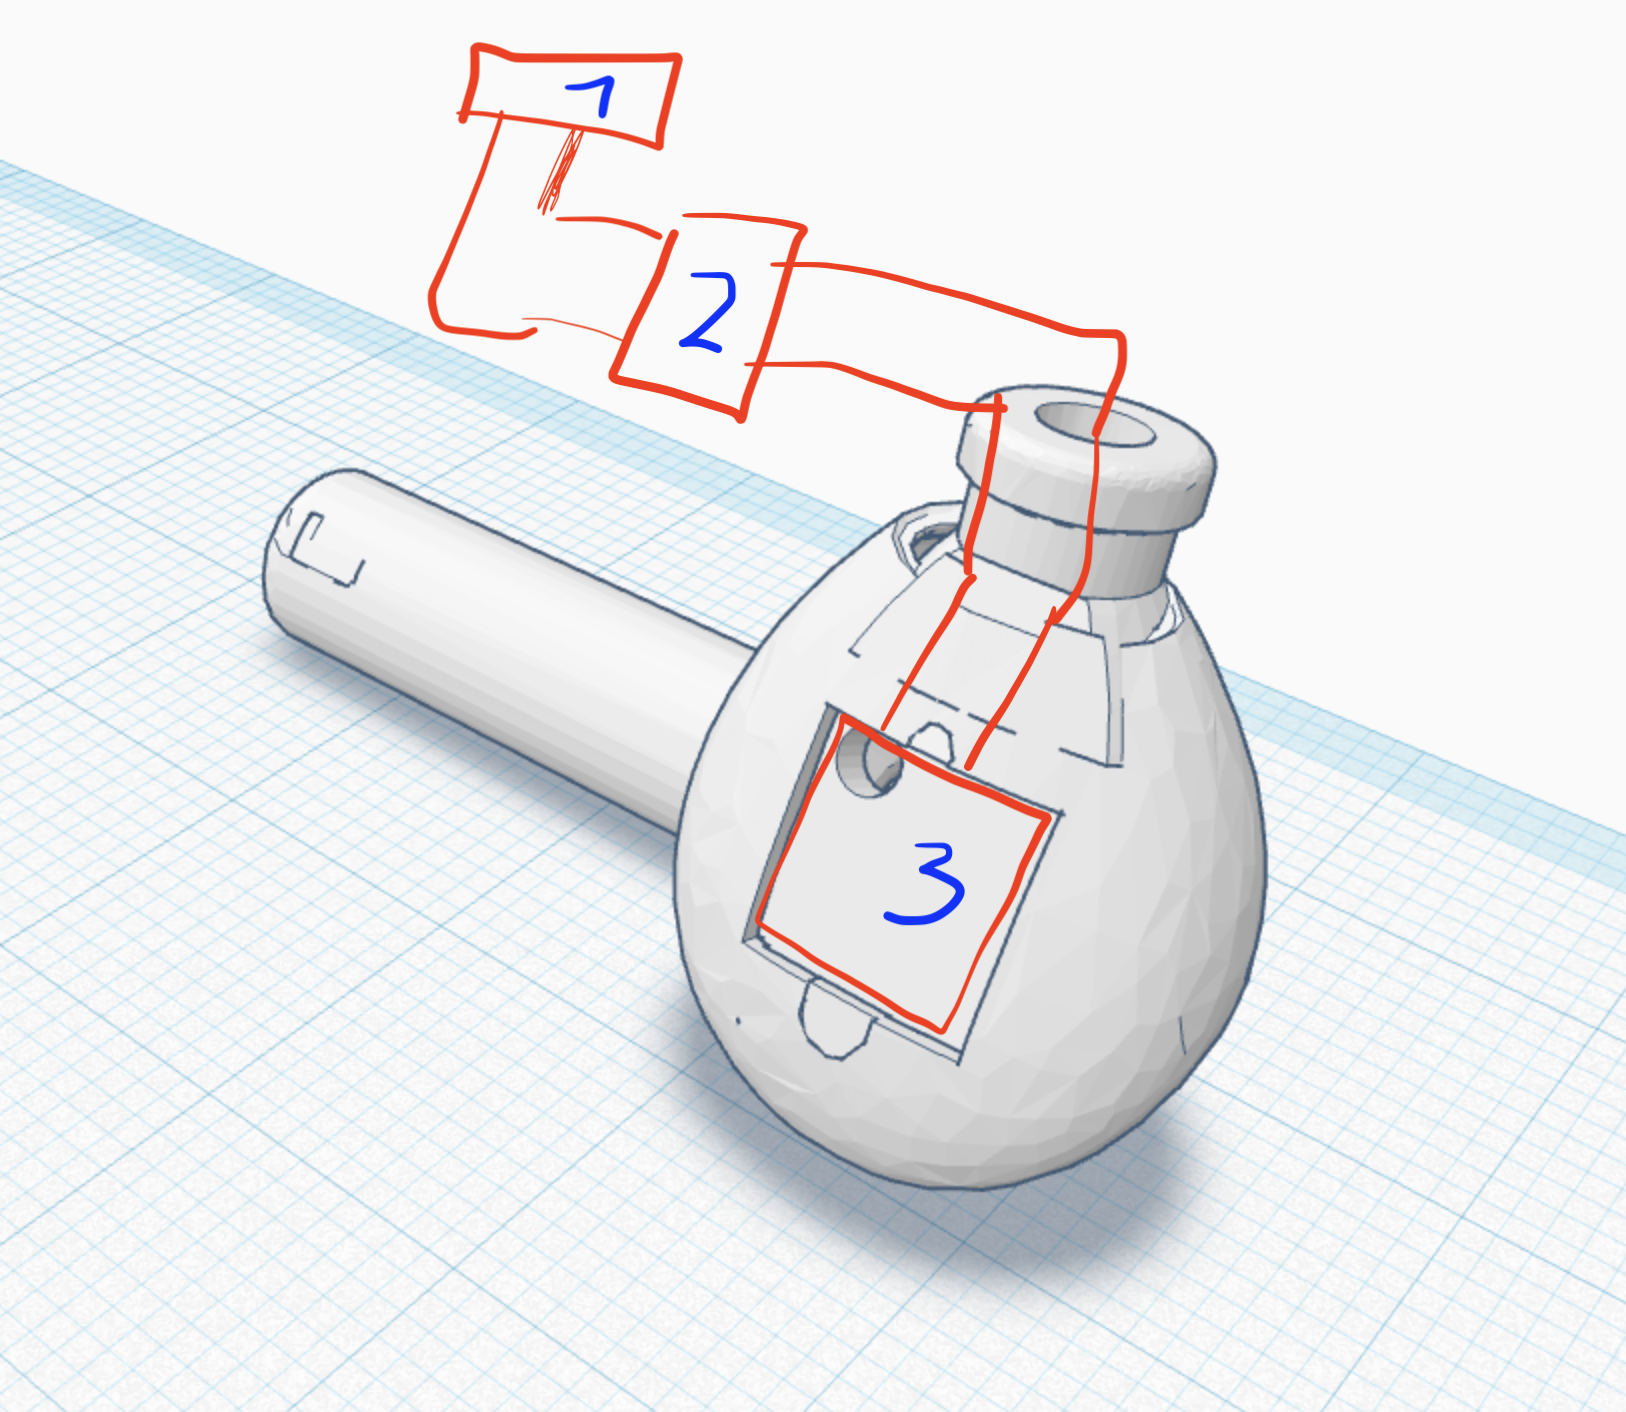
\includegraphics[width=0.9\linewidth]{../thesis-doc/images/prototype/flex_pcb_design_finding.png}
    \end{column}

    \begin{column}{.48\textwidth}
      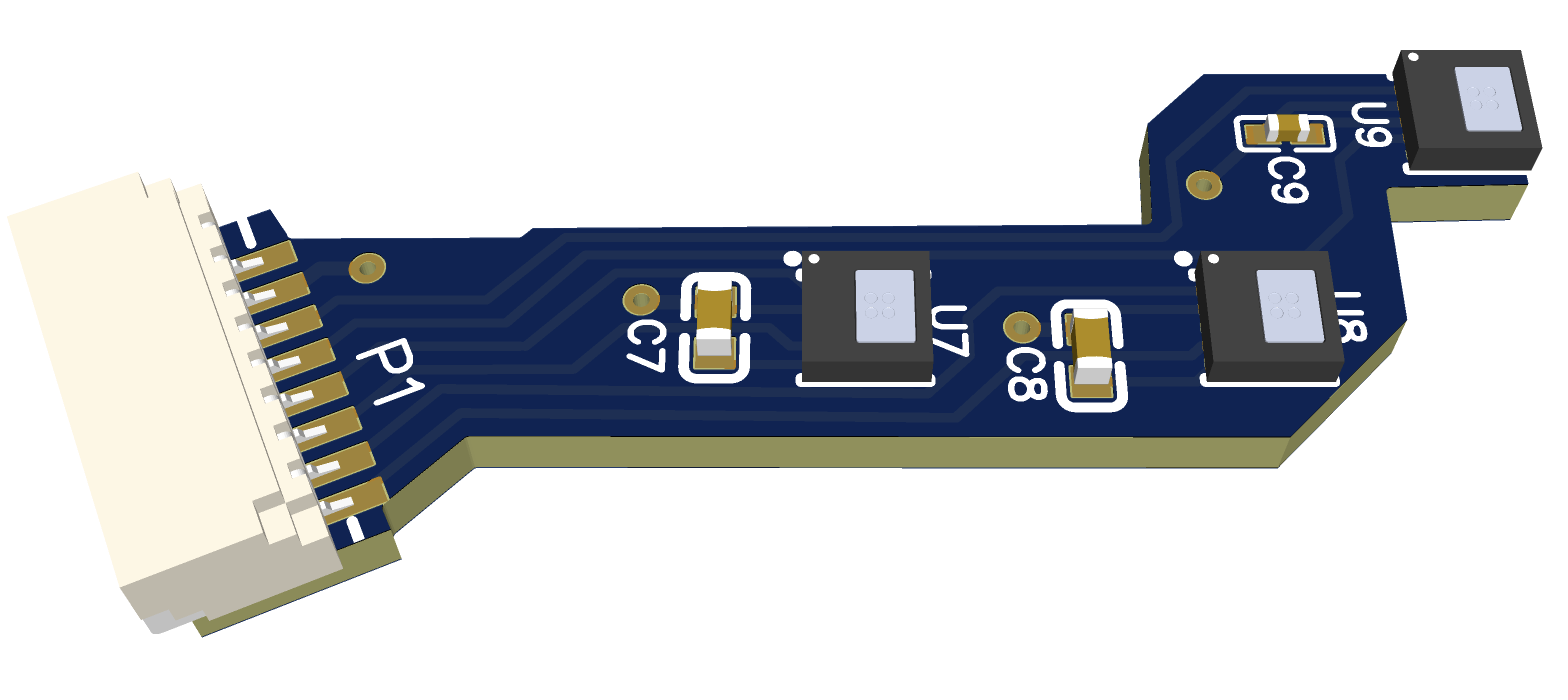
\includegraphics[width=1.05\linewidth]{../thesis-doc/images/prototype/pcb/flex_pcb_3D.png}
    \end{column}
  \end{columns}
    
\end{frame}

% \begin{frame}{Prototype: FlexPCB}
%   \begin{columns}[T]
%     \begin{column}{.31\textwidth}
%       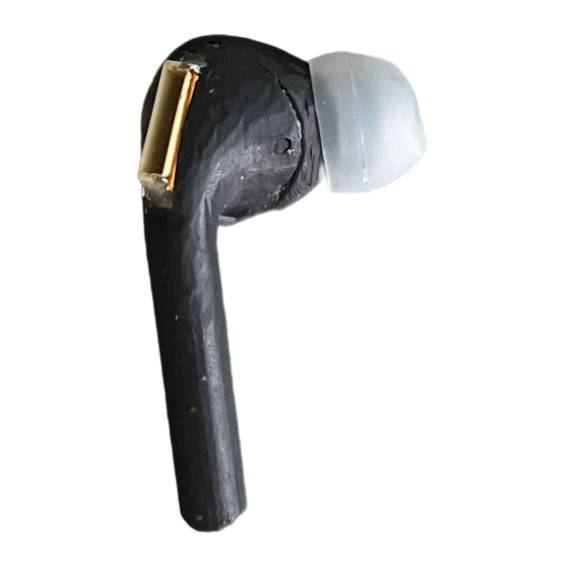
\includegraphics[width=0.9\linewidth]{../thesis-doc/images/prototype/Earpod_Side1.png}
%     \end{column}
    
%     \begin{column}{.31\textwidth}
%       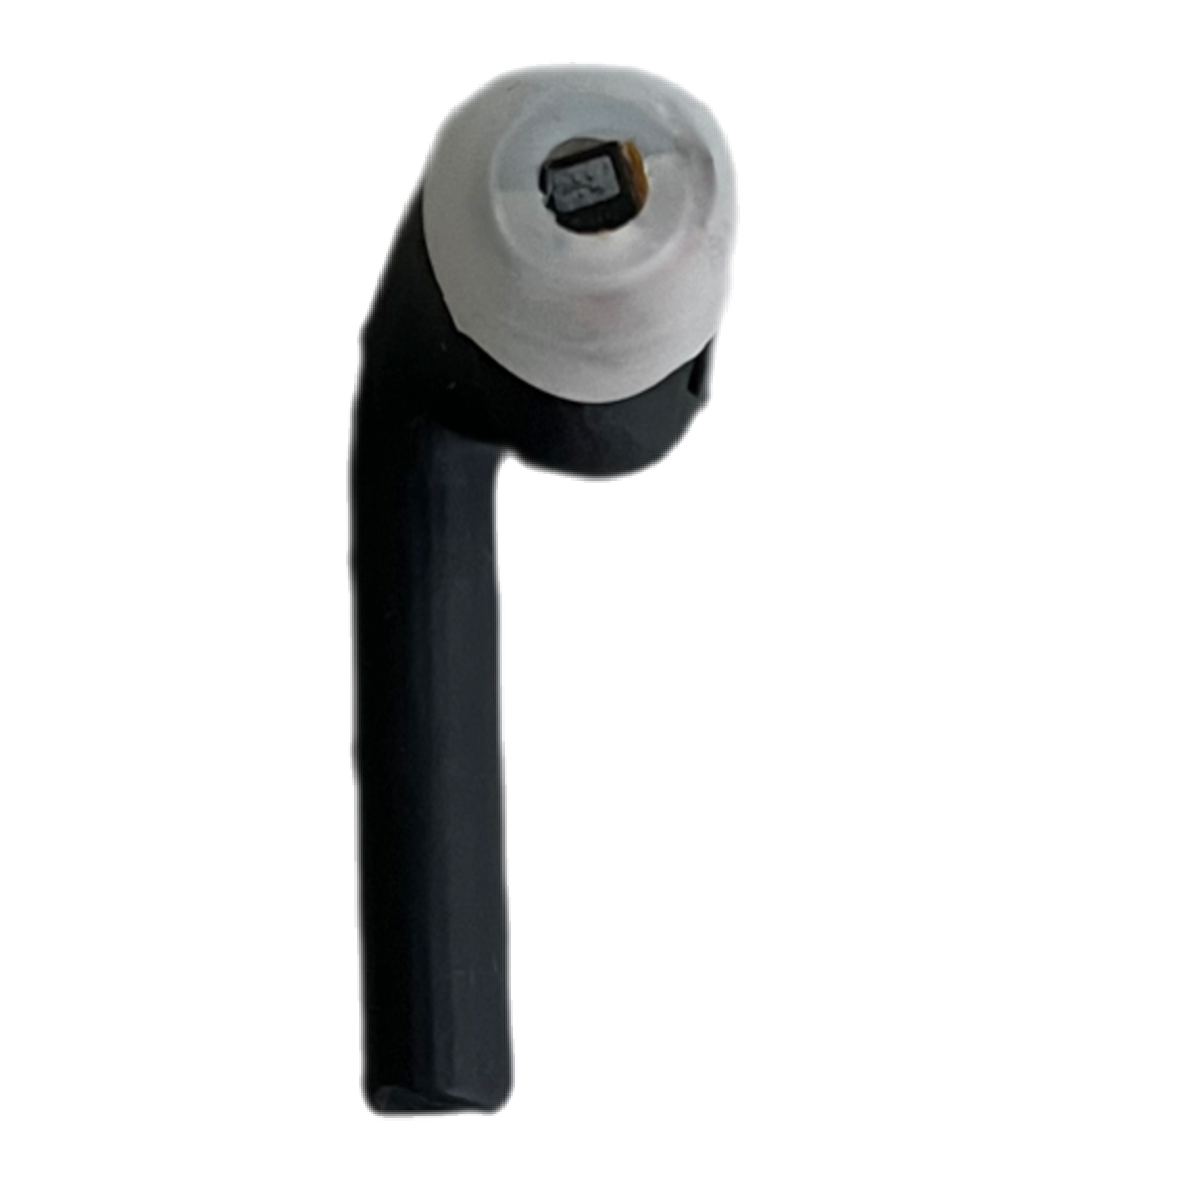
\includegraphics[width=0.9\linewidth]{../thesis-doc/images/prototype/Earpod_Front_2.pdf}
%     \end{column}
    
%     \begin{column}{.31\textwidth}
%       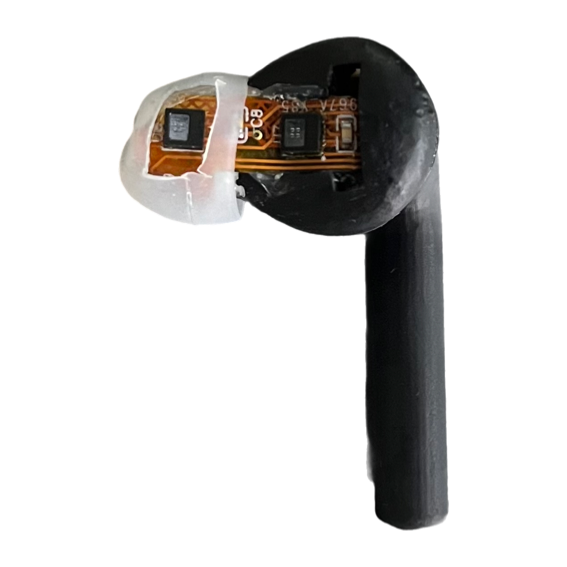
\includegraphics[width=0.9\linewidth]{../thesis-doc/images/prototype/Earpod_Side2.png}
%     \end{column}
%   \end{columns}
% \end{frame}

\begin{frame}{Prototype: FlexPCB}
  \begin{columns}[T]
    \begin{column}{.31\textwidth}
      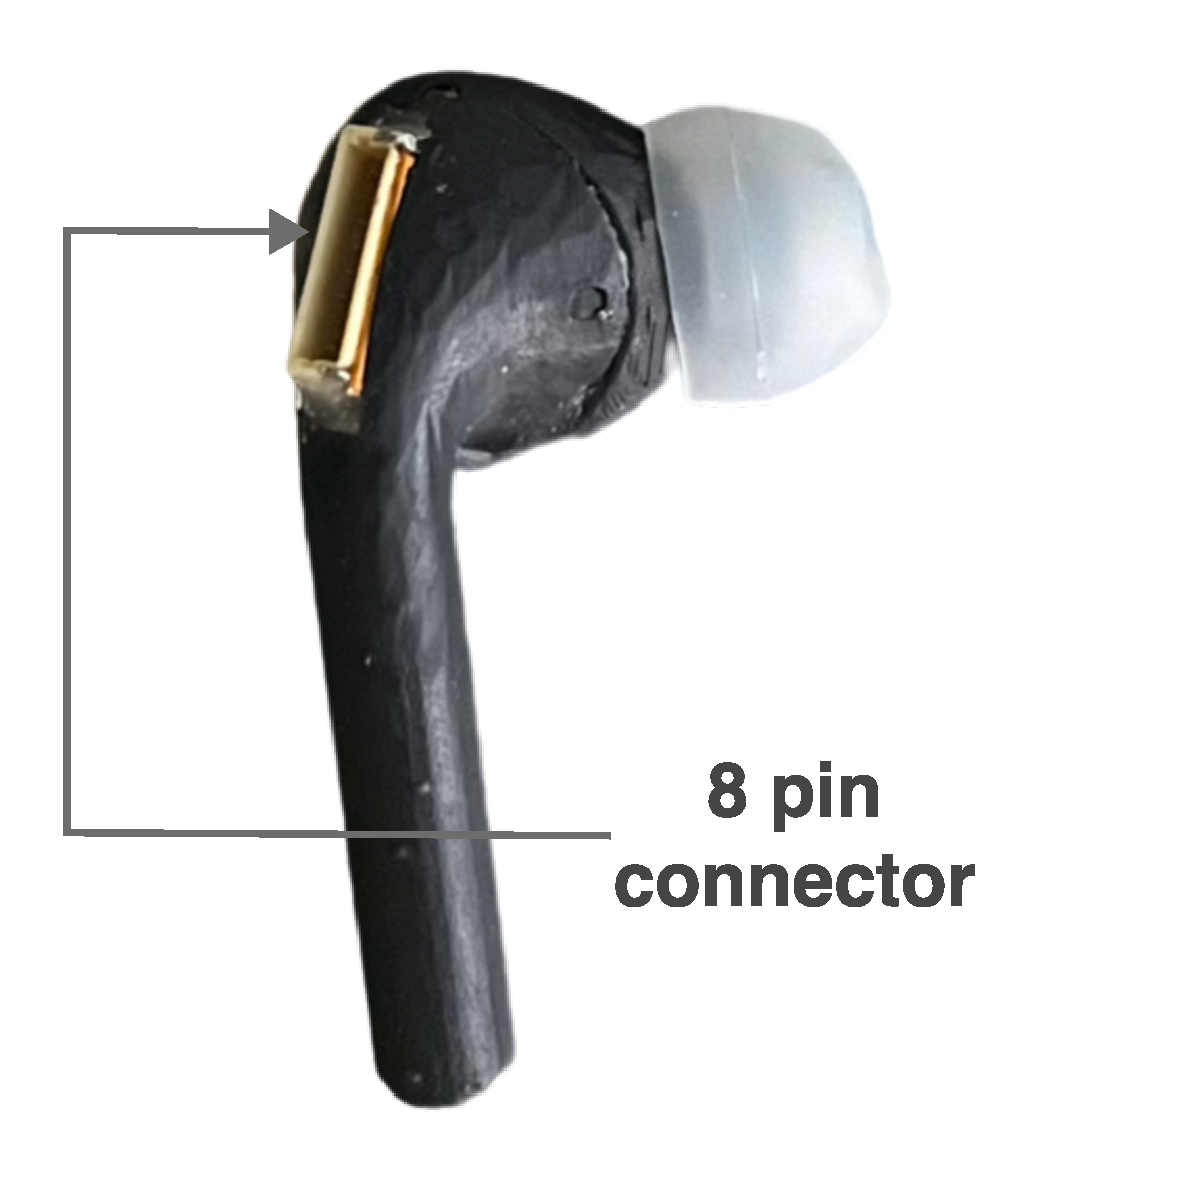
\includegraphics[width=0.9\linewidth]{../thesis-doc/images/prototype/Earpod_Side1_visual_markers.pdf}
    \end{column}
    
    \begin{column}{.31\textwidth}
      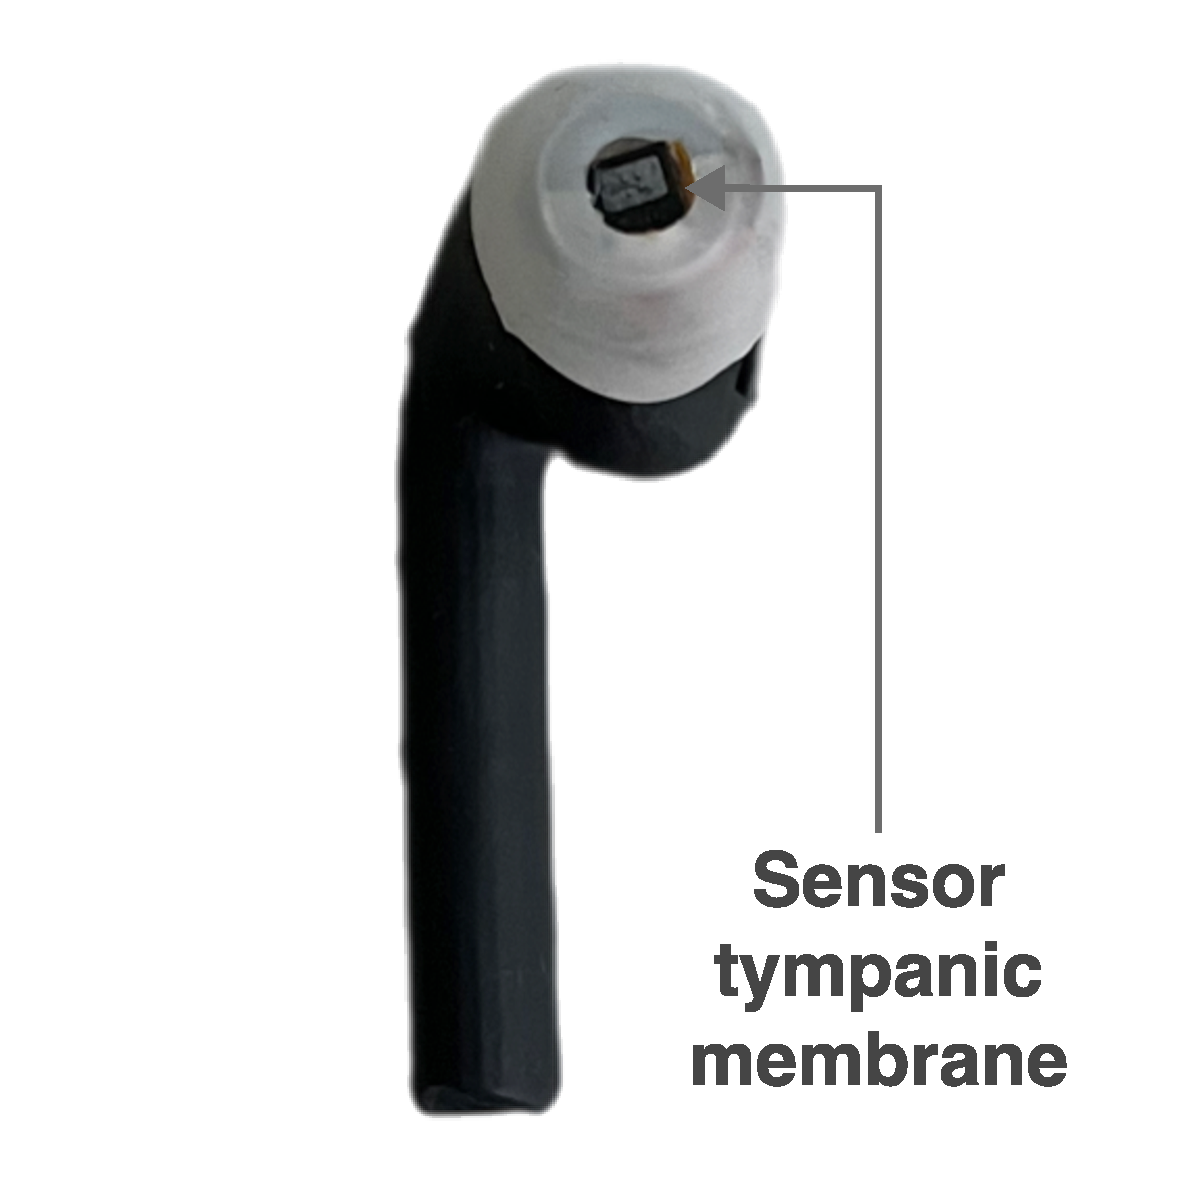
\includegraphics[width=0.9\linewidth]{../thesis-doc/images/prototype/Earpod_Front_visual_markers.pdf}
    \end{column}

    \begin{column}{.31\textwidth}
      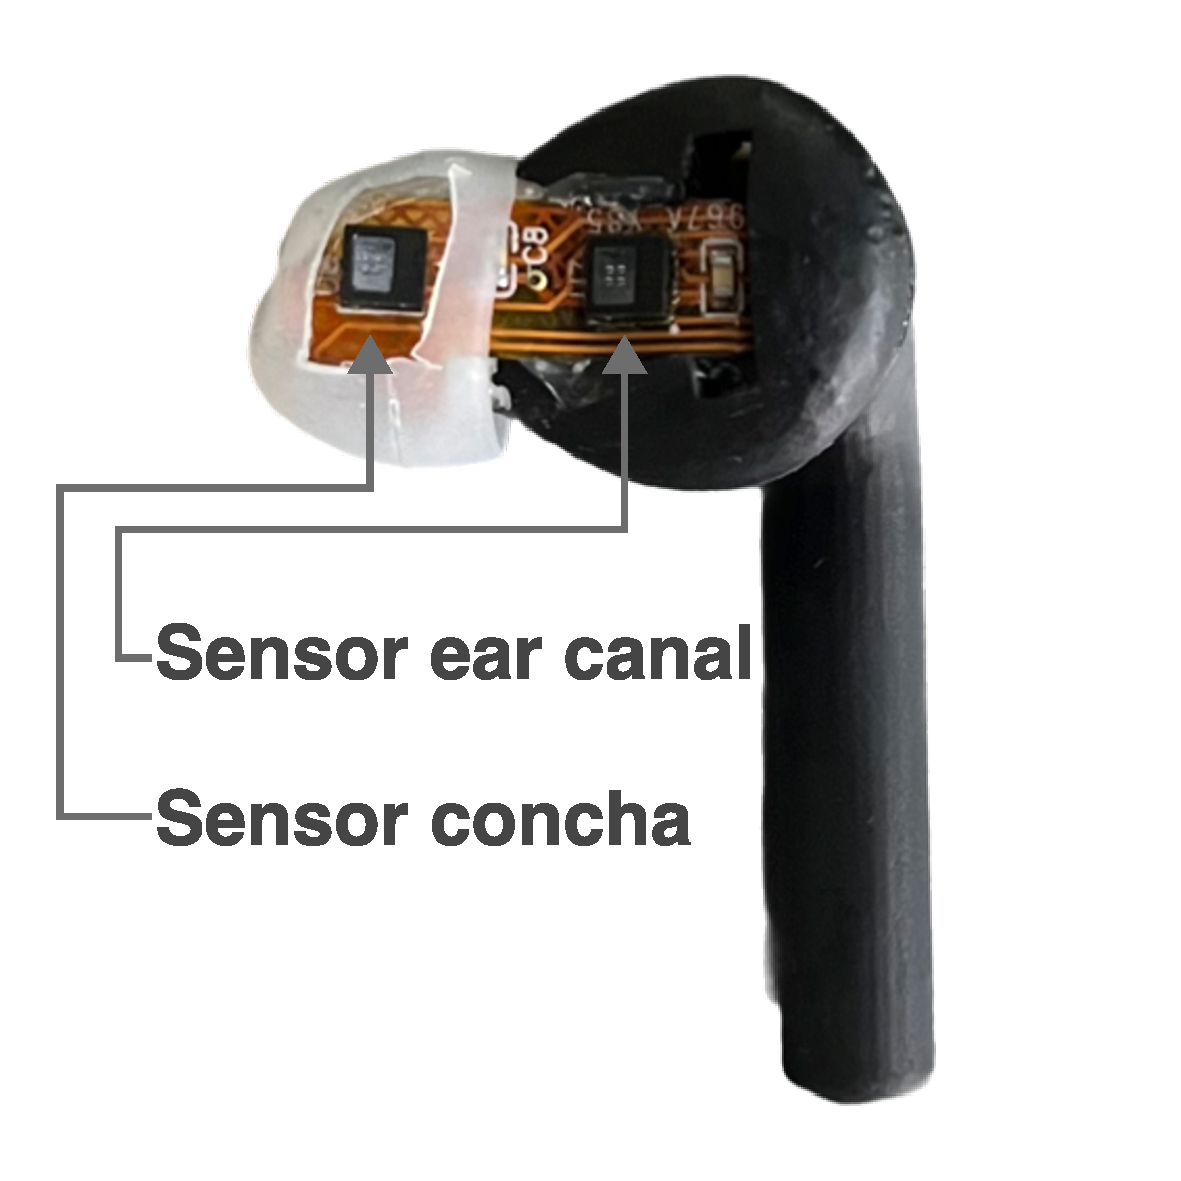
\includegraphics[width=0.9\linewidth]{../thesis-doc/images/prototype/Earpod_Side2_visual_markers.pdf}
    \end{column}
  \end{columns}
\end{frame}

\section{Study 1}
\begin{frame}{Study 1: Localized Ear Temperature Measurement Study Procedure: Baseline Surveys and Environmental Influences}
    \begin{itemize}
        \item 12 probands (7 male, 5 female)
        \item Mean room temperature $25.4^\circ\text{C}$
        \item Mean outdoor temperature: $19.4^\circ\text{C}$
        \item Thermometer measurement before/after data measurement
    \end{itemize}
    \begin{center}
        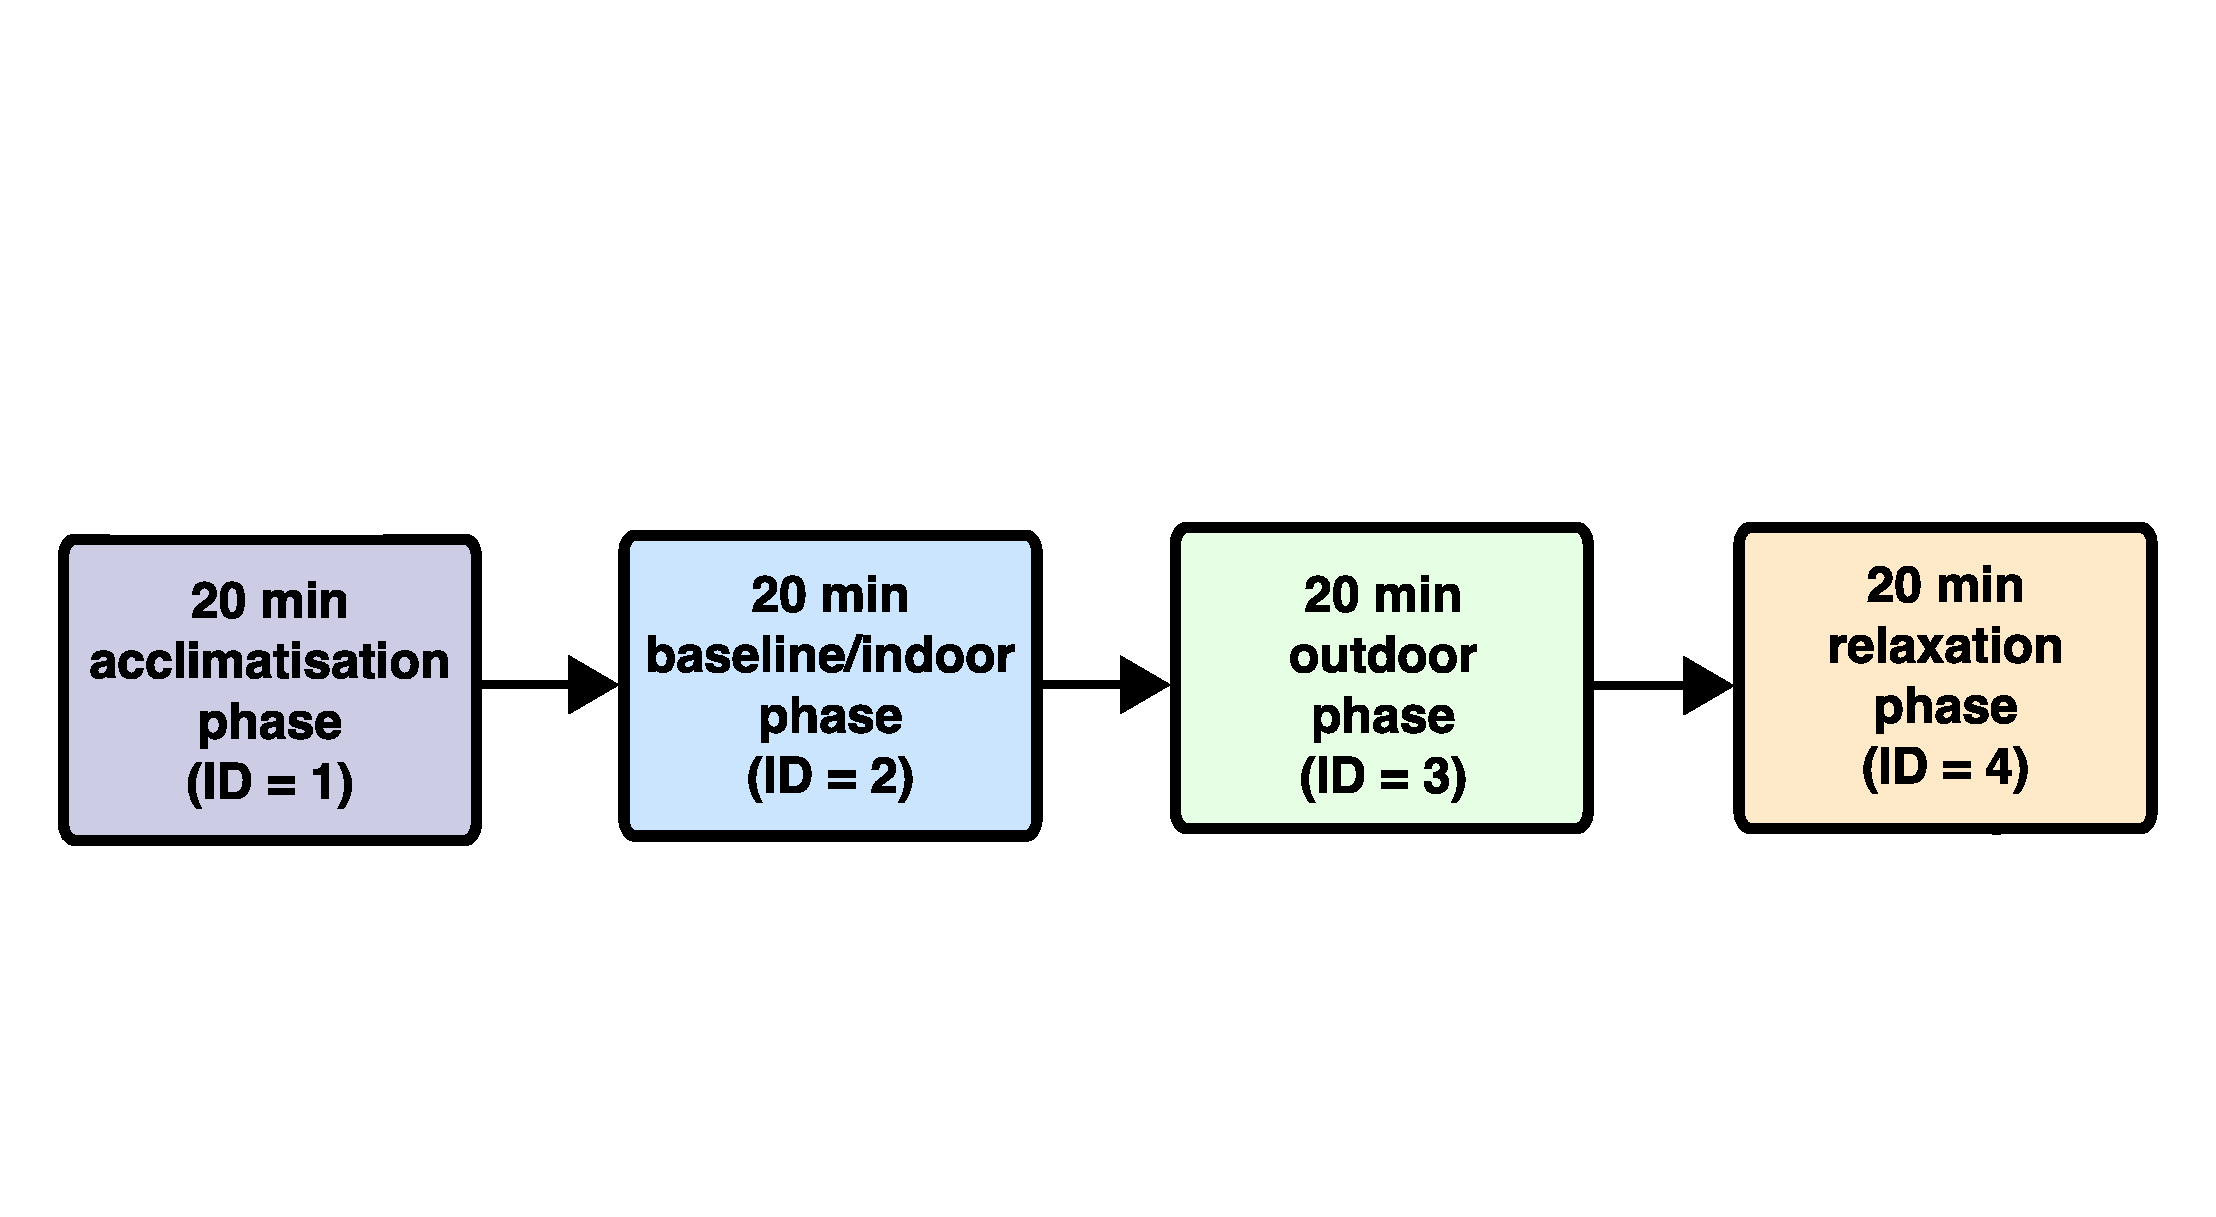
\includegraphics[width=0.95\linewidth]{../thesis-doc/images/study1/Procedure_short.pdf}
    \end{center}
\end{frame}

\begin{frame}
    \begin{center}
        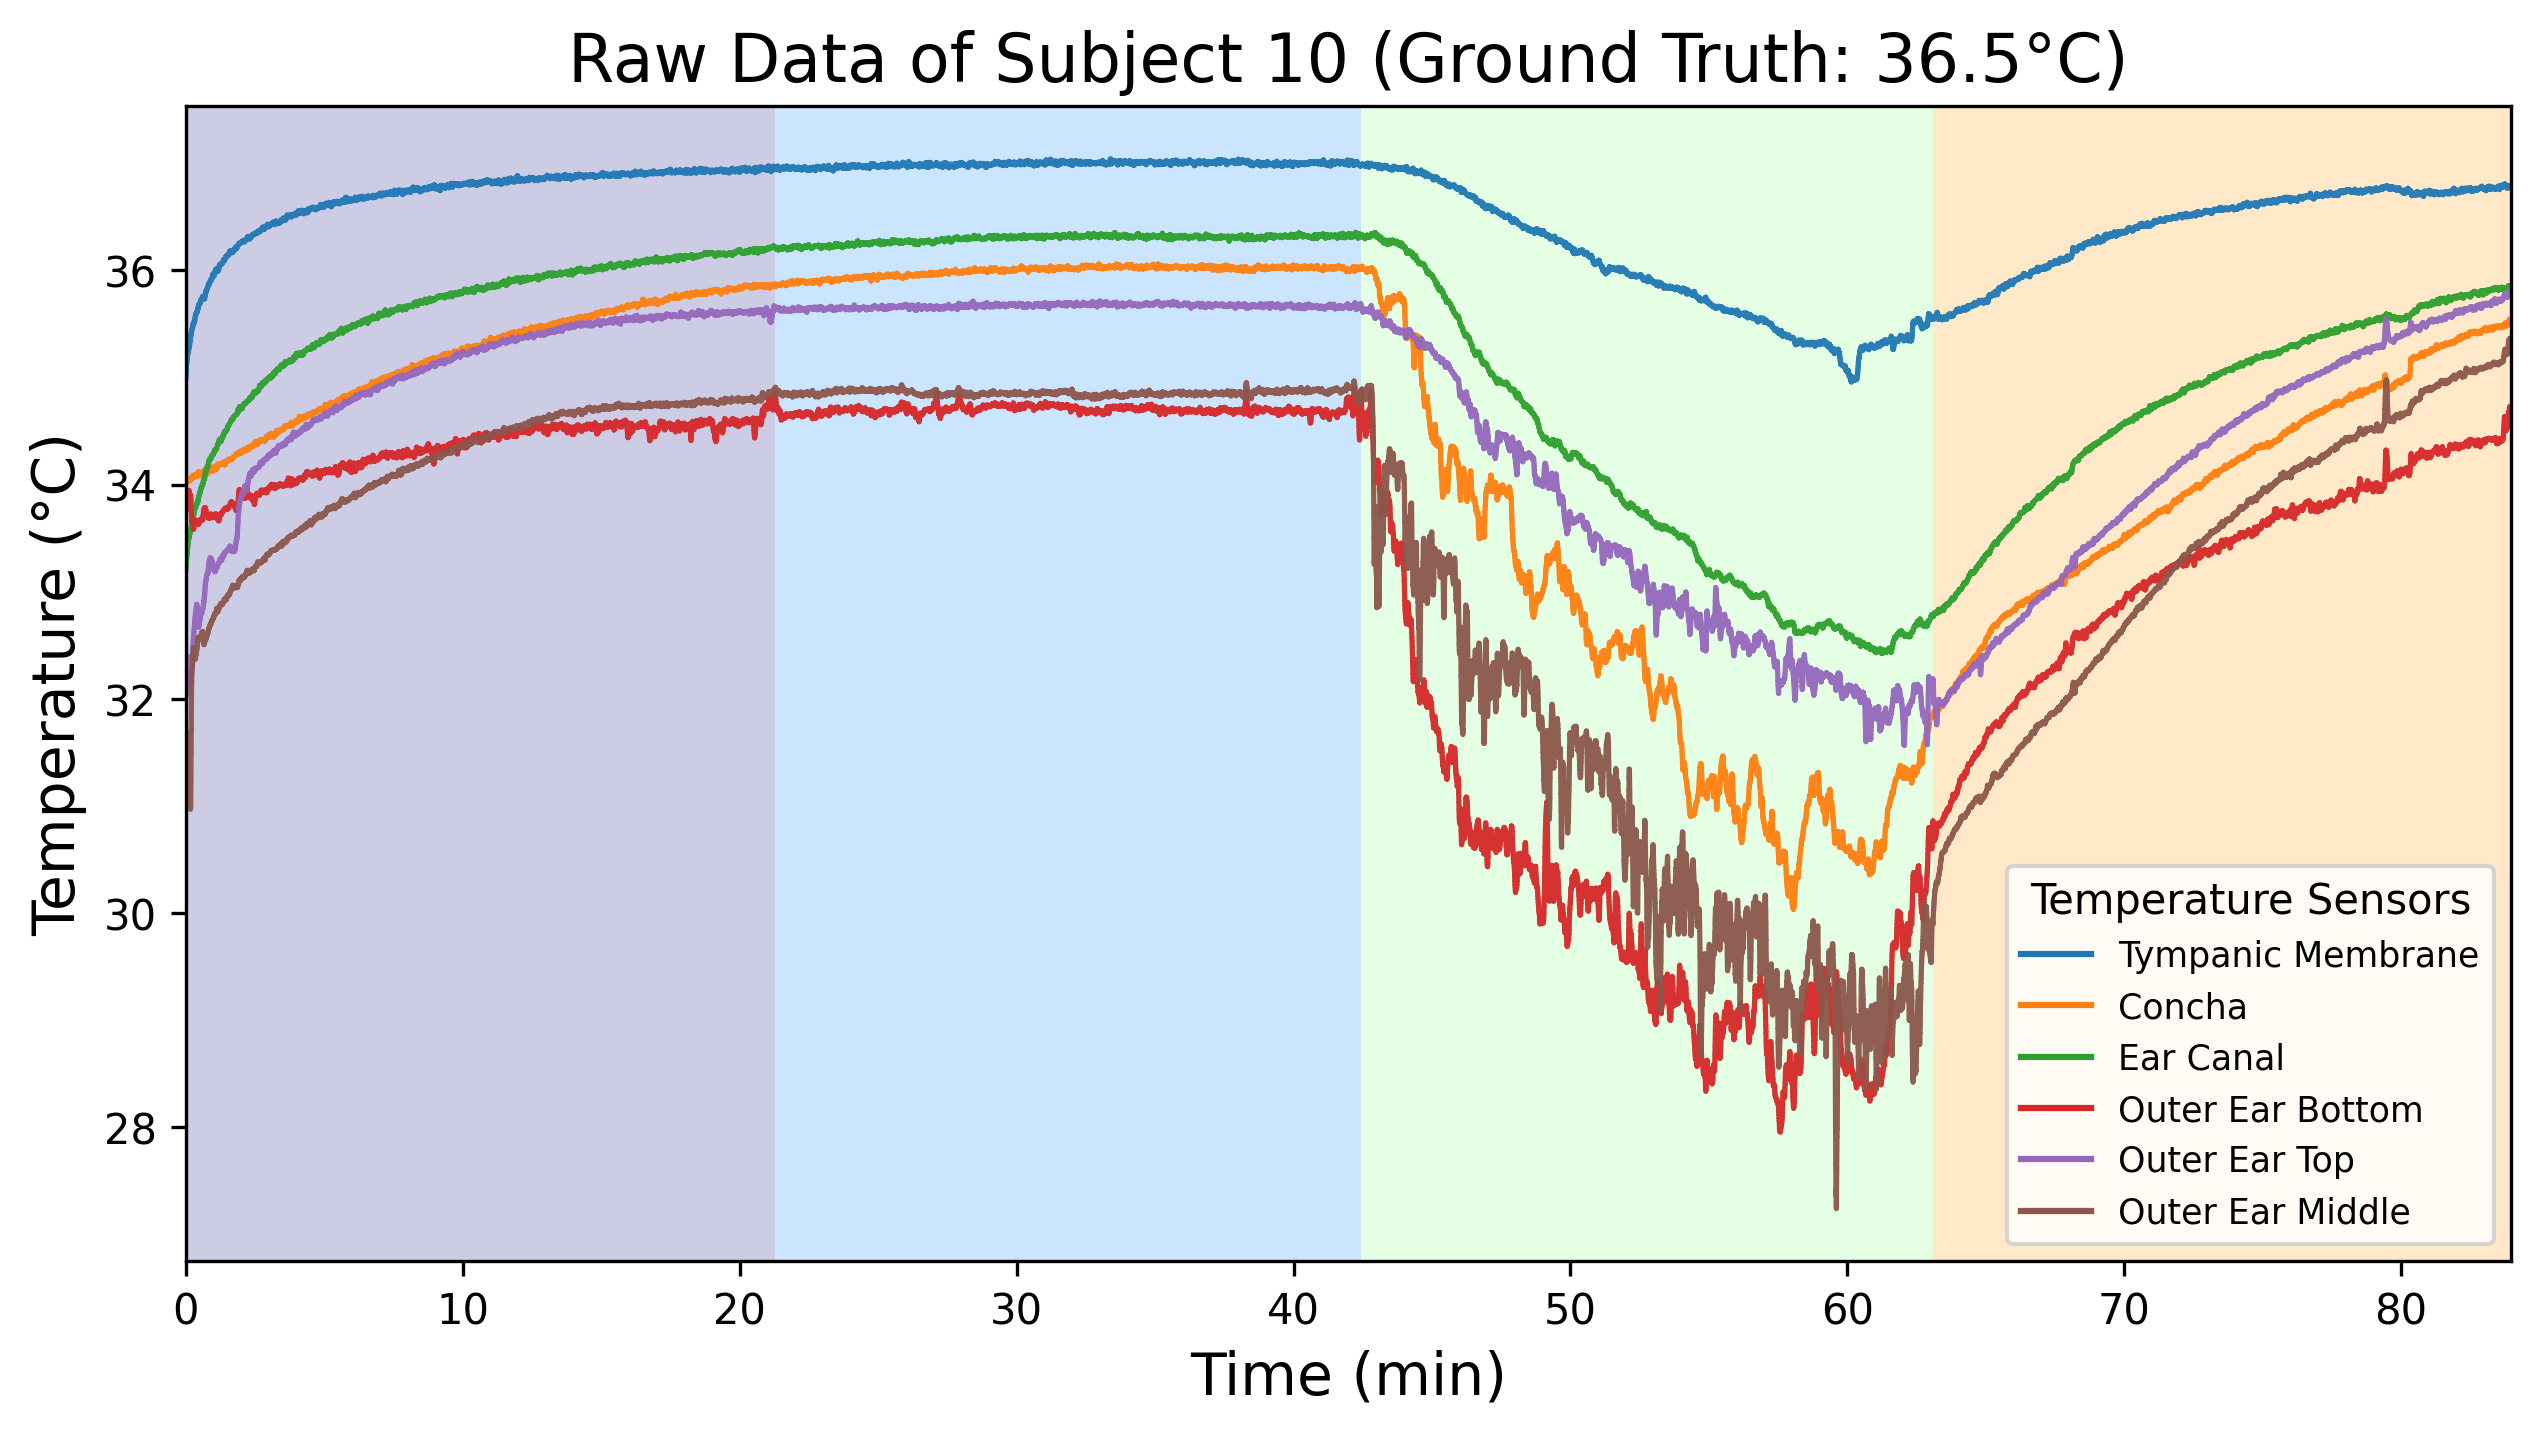
\includegraphics[width=0.9\linewidth]{../thesis-doc/images/study1/Logging_person_10_0smoothed_raw_data.png}
    \end{center}
\end{frame}

\begin{frame}{Evaluation Study 1: Hypothesis 1}
    \textbf{The temperature measured by sensors located behind the ear is lower compared to the other locations.}
    \begin{center}
      \begin{columns}[T]
        \begin{column}{.3\textwidth}
        \vspace{10pt}
          \begin{itemize}
              \item Baseline phase (phase 2)
              \item Mean temperature of all probands
              \begin{itemize}
                  \item The ground truth is subtracted from each measured temperature value
              \end{itemize}
          \end{itemize}
        \end{column}
        
        \begin{column}{.66\textwidth}
        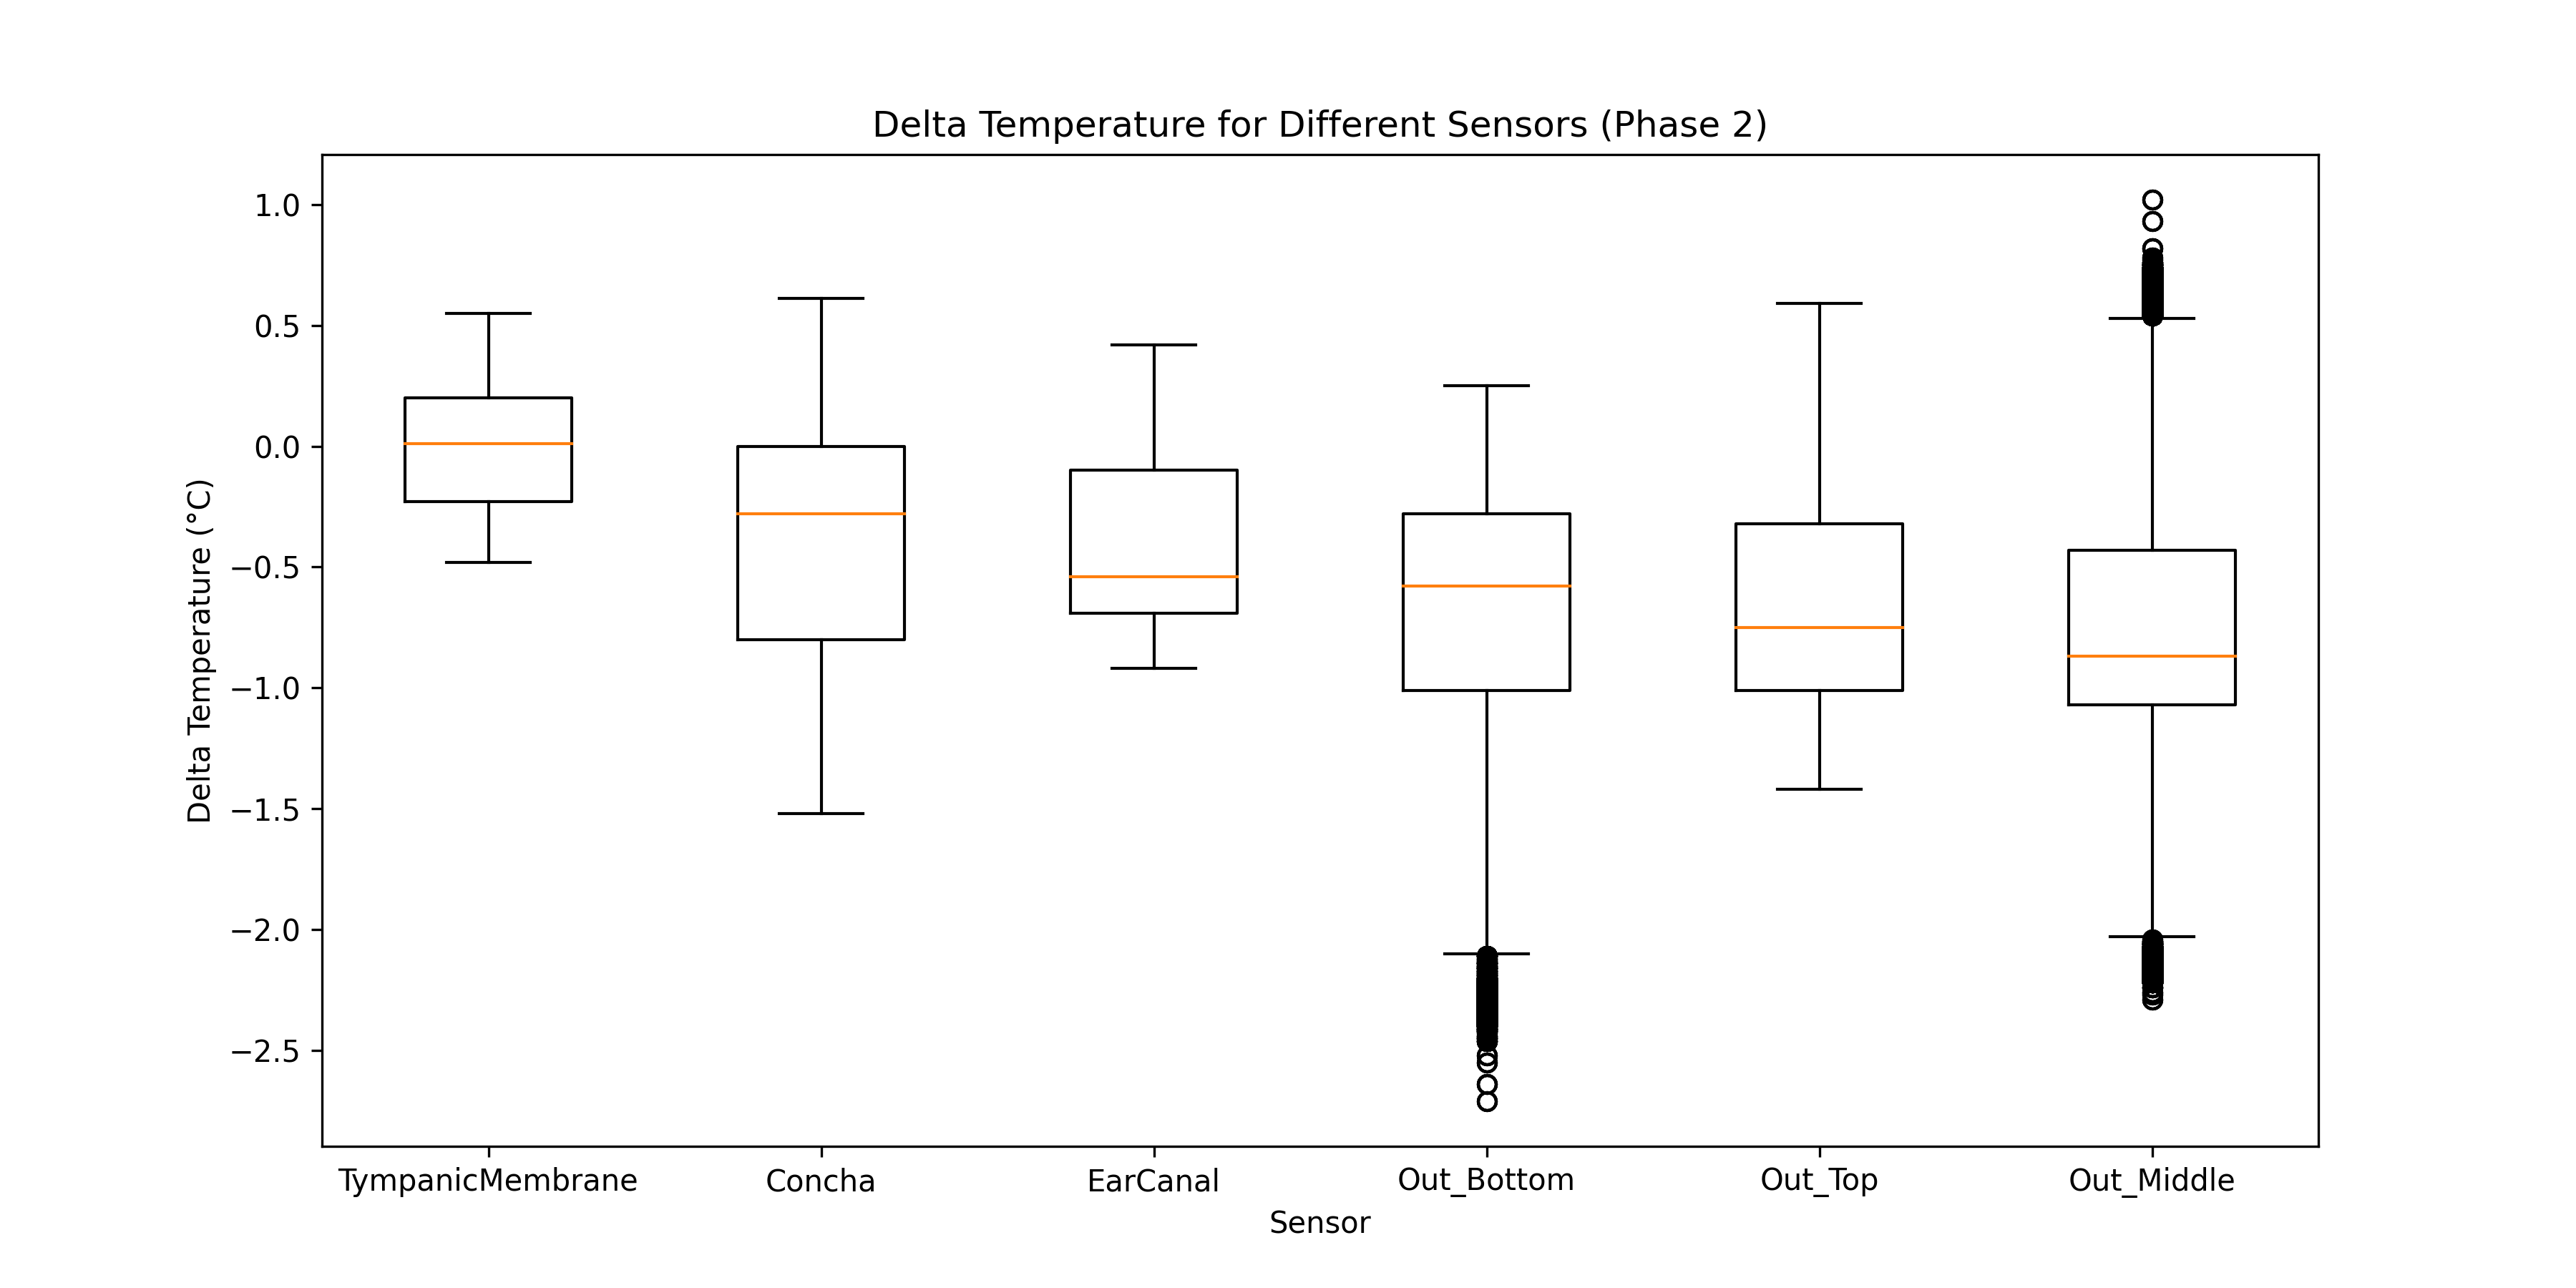
\includegraphics[width=0.99\linewidth]{../thesis-doc/images/study1/hypothesis1/hypothesis1_boxplot_phase_2.png}
        \end{column}
      \end{columns}
    \end{center}
\end{frame}

\begin{frame}{Evaluation Study 1: Hypothesis 1}
    \textbf{The temperature measured by sensors located behind the ear is lower compared to the other locations.}
    \begin{center}
      \begin{columns}[T]
        \begin{column}{.3\textwidth}
        \vspace{10pt}
          \begin{itemize}
              \item Outdoor phase (phase 3)
              \item Mean temperature of all probands
              \begin{itemize}
                  \item The ground truth is subtracted from each measured temperature value
              \end{itemize}
          \end{itemize}
        \end{column}
        
        \begin{column}{.66\textwidth}
        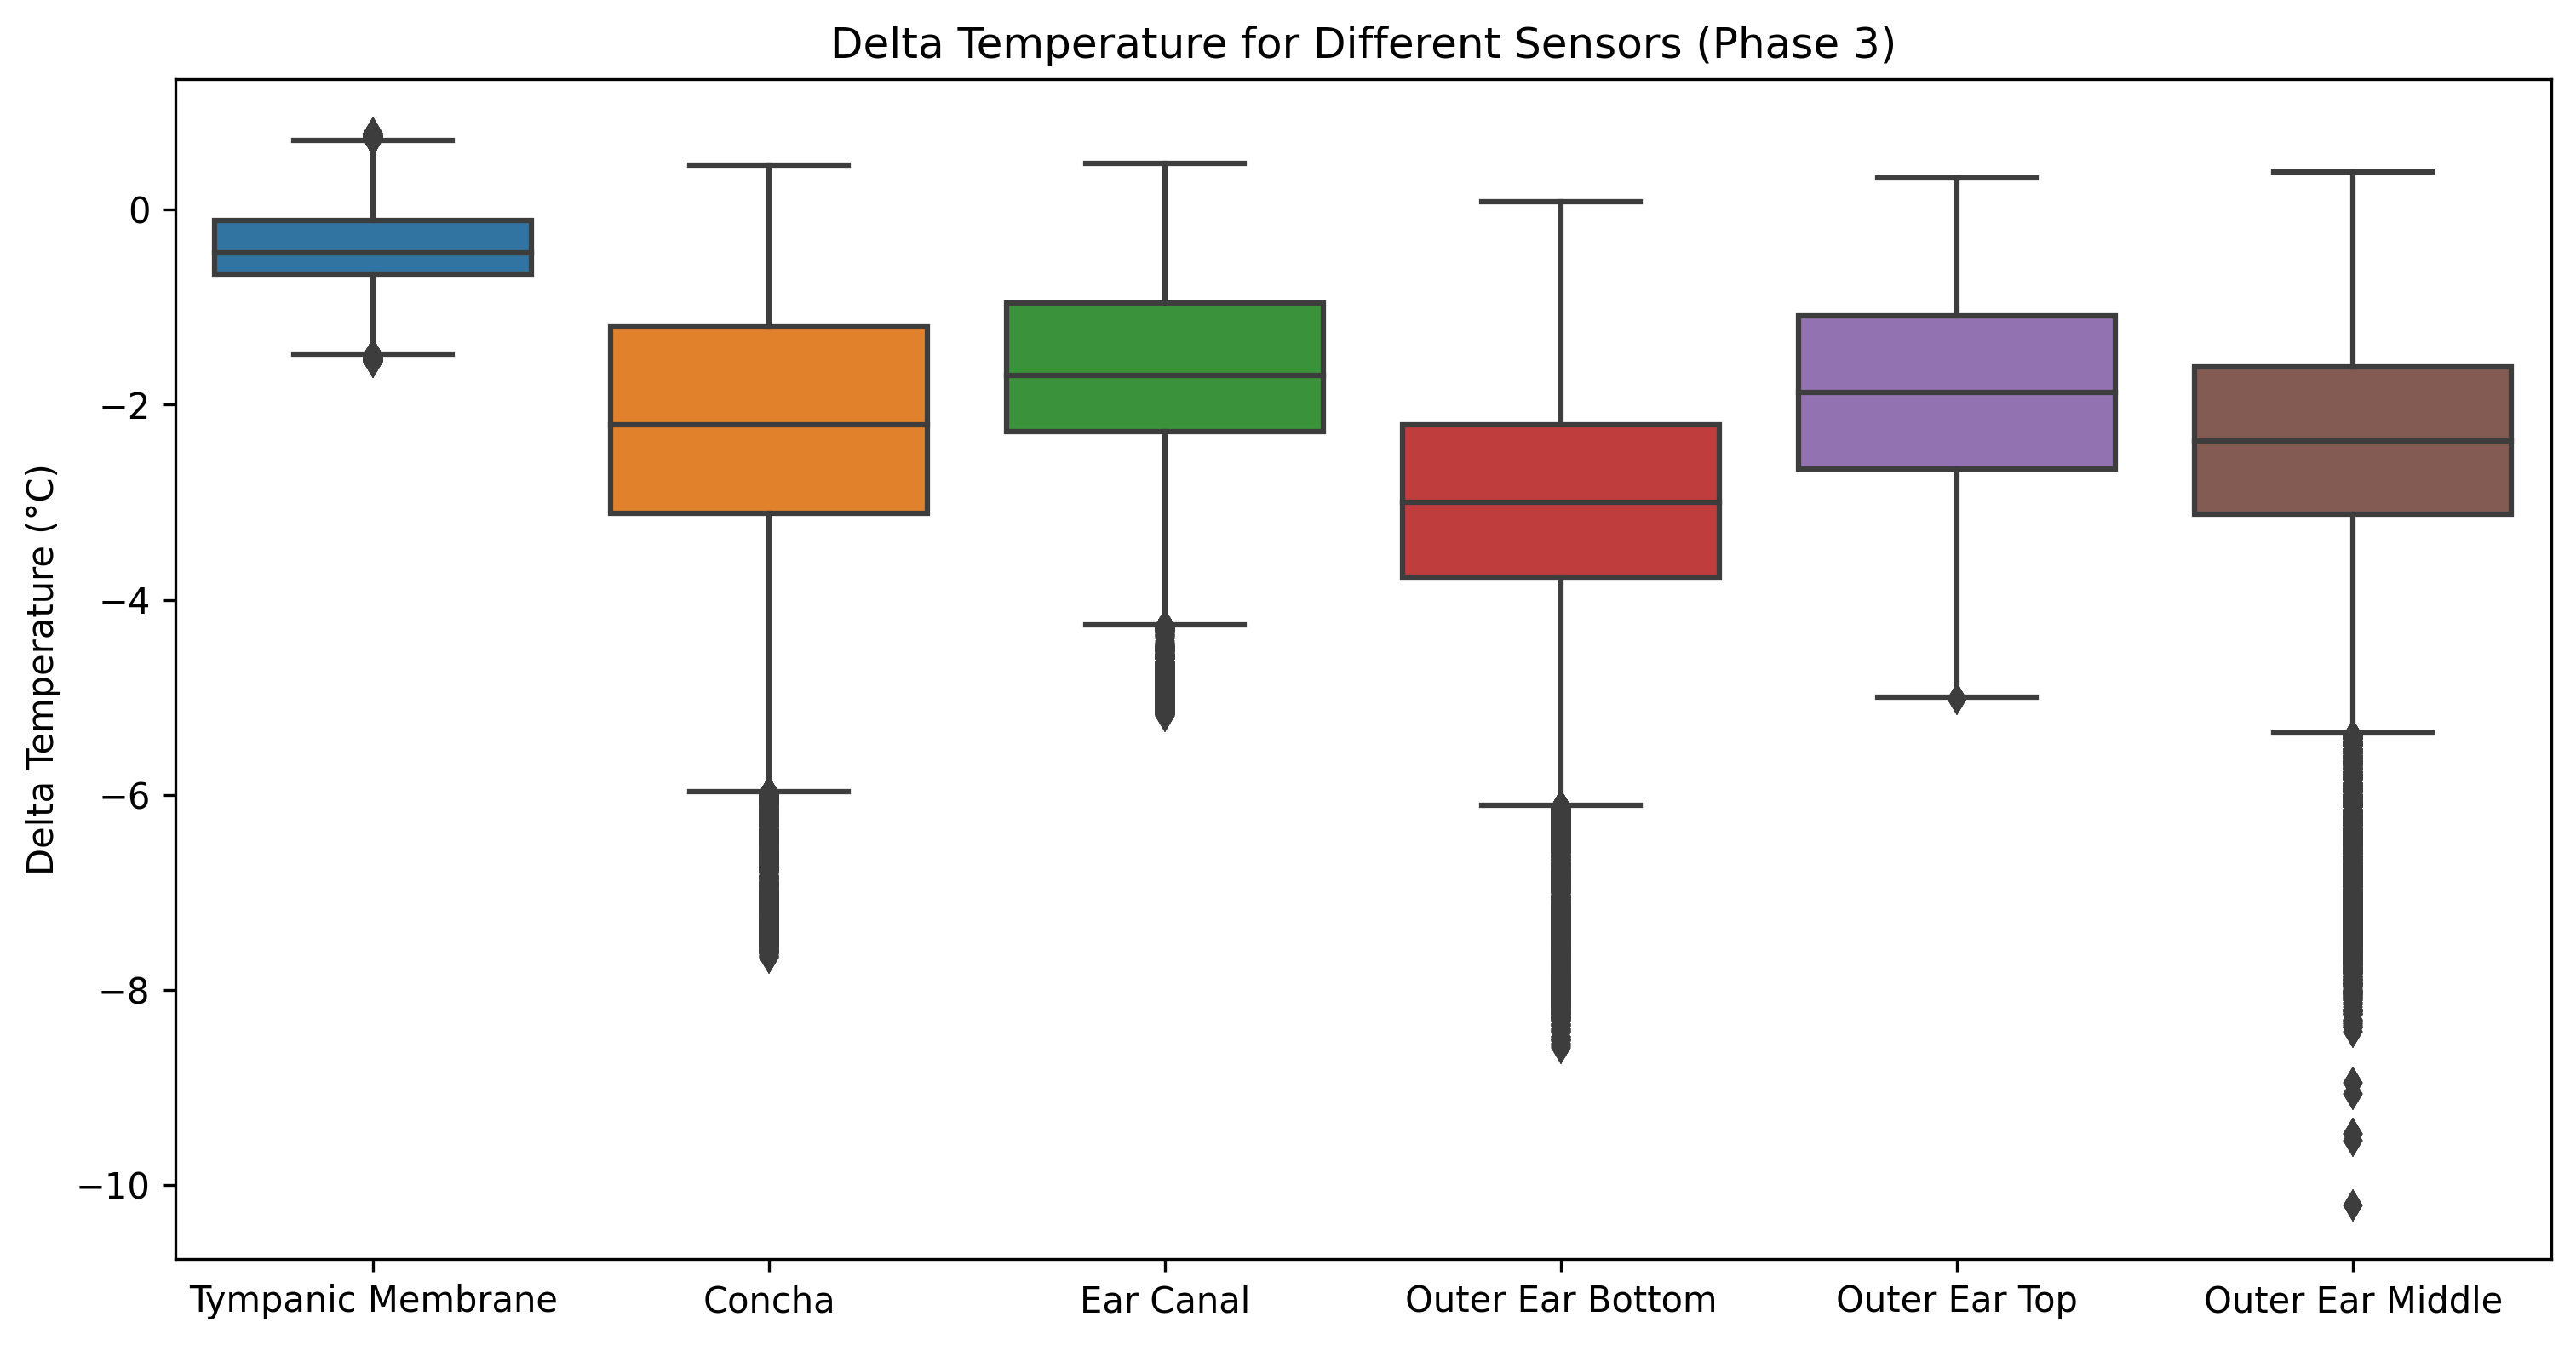
\includegraphics[width=0.99\linewidth]{../thesis-doc/images/study1/hypothesis1/hypothesis1_boxplot_phase_3.png}
        \end{column}
      \end{columns}
    \end{center}
\end{frame}

\begin{frame}{Evaluation Study 1: Hypothesis 2}
    \textbf{The variance in temperature readings differs between indoor and outdoor settings}

    \begin{itemize}
        \item Huge increase in variance between indoor and outdoor phase for each sensor position
    \end{itemize}
    \vspace{15pt}
    \begin{tabularx}{\textwidth}{|X|c|c|}
        \hline
        \textbf{Sensor} & \multicolumn{2}{c|}{\textbf{Mean Variance}} \\
         & \multicolumn{2}{c|}{\textbf{(in ^\circ \text{C}^2)}} \\
         & \textbf{Indoor} & \textbf{Outdoor} \\
        \hline
        \textbf{Tympanic Membrane} & 0.00097 & 0.107 \\
        \textbf{Concha} & 0.00307 & 1.134 \\
        \textbf{EarCanal} & 0.00155 & 0.646 \\
        \textbf{Outer Ear Bottom} & 0.01890 & 1.110 \\
        \textbf{Outer Ear Top} & 0.00694 & 0.650 \\
        \textbf{Outer Ear Middle} & 0.01980 & 1.098 \\
        \hline
    \end{tabularx}
\end{frame}

\begin{frame}{Evaluation Study 1: Hypothesis 2}
    \textbf{The variance in temperature readings differs between indoor and outdoor settings}

    \begin{itemize}
        \item Null hypothesis is rejected, if $p<0.05$.
        \item Strong indication that the hypothesis is proven.
    \end{itemize}
    \vspace{15pt}
    \begin{tabularx}{\textwidth}{|X|c|}
\hline
\textbf{Sensor} & \textbf{p-value} \\
\hline
Tympanic Membrane & \(0.0005438\) \\
Concha & \(0.0005870\) \\
Ear Canal & \(0.0005009\) \\
Outer Ear Bottom & \(4.71 \times 10^{-6}\) \\
Outer Ear Top & \(7.04 \times 10^{-7}\) \\
Outer Ear Middle & \(0.0002436\) \\
\hline
\end{tabularx}
\end{frame}


% \begin{frame}{Evaluation Study 1: Hypothesis 3}
%     \begin{itemize}
%         \item additional info or pictures
%     \end{itemize}
% \end{frame}

\begin{frame}{Evaluation Study 1: Hypothesis 4}
    \textbf{The temperature at the tympanic membrane has the greatest stability compared to other sensor locations}
    \begin{itemize}
        \item The results for the outdoor area in particular show that the tympanic membrane is the most stable.
    \end{itemize}
    \vspace{15pt}
    
        \begin{tabularx}{\textwidth}{|X|c|c|}
        \hline
        \textbf{Sensor} & \textbf{Mean Standard Deviation} & \textbf{Mean Standard Deviation} \\
        & \textbf{Phase 2 (indoor)} & \textbf{Phase 3 (outdoor)} \\
        \hline
        \textbf{Tympanic Membrane} & 0.0308 & 0.3048 \\
        \textbf{Concha} & 0.0535 & 0.9882 \\
        \textbf{Ear Canal} & 0.0378 & 0.7496 \\
        \textbf{Outer Ear Bottom} & 0.1138 & 1.0156 \\
        \textbf{Outer Ear Top} & 0.0730 & 0.7836 \\
        \textbf{Outer Ear Middle} & 0.1176 & 0.9875 \\
        \hline
        \end{tabularx}
\end{frame}

\begin{frame}{Evaluation Study 1: Hypothesis 4}
    \textbf{The temperature at the tympanic membrane has the greatest stability compared to other sensor locations}
    \begin{itemize}
        \item Null hypothesis is rejected if $p<0.05$.
        \item Strong indication that the hypothesis is proven.
    \end{itemize}
    \vspace{15pt}
    
    \begin{tabularx}{\textwidth}{|X|c|}
        \hline
        \textbf{Sensor} & \textbf{p-value} \\
        \hline
        Tympanic Membrane & \(1.25 \times 10^{-5}\) \\
        Concha & \(9.39 \times 10^{-6}\) \\
        Ear Canal & \(5.96 \times 10^{-6}\) \\
        Outer Ear Bottom & \(2.09 \times 10^{-7}\) \\
        Outer Ear Top & \(6.59 \times 10^{-8}\) \\
        Outer Ear Middle & \(2.71 \times 10^{-6}\) \\
        \hline
        \end{tabularx}
\end{frame}

% \begin{frame}{Evaluation Study 1: Hypothesis 5}
%     \begin{itemize}
%         \item additional info or pictures
%     \end{itemize}
% \end{frame}

\section{Study 2}
\begin{frame}{Study 2: Study Course Under Stress Conditions: Impact on Temperature Measurements With Ear-Based Sensors}
    \begin{itemize}
        \item 5 probands (3 male, 2 female)
        \item Mean room temperature $23.1^\circ\text{C}$
        \item Thermometer measurement before/after data measurement
        \item Polar H9 as ground truth for stress
    \end{itemize}
\begin{center}
  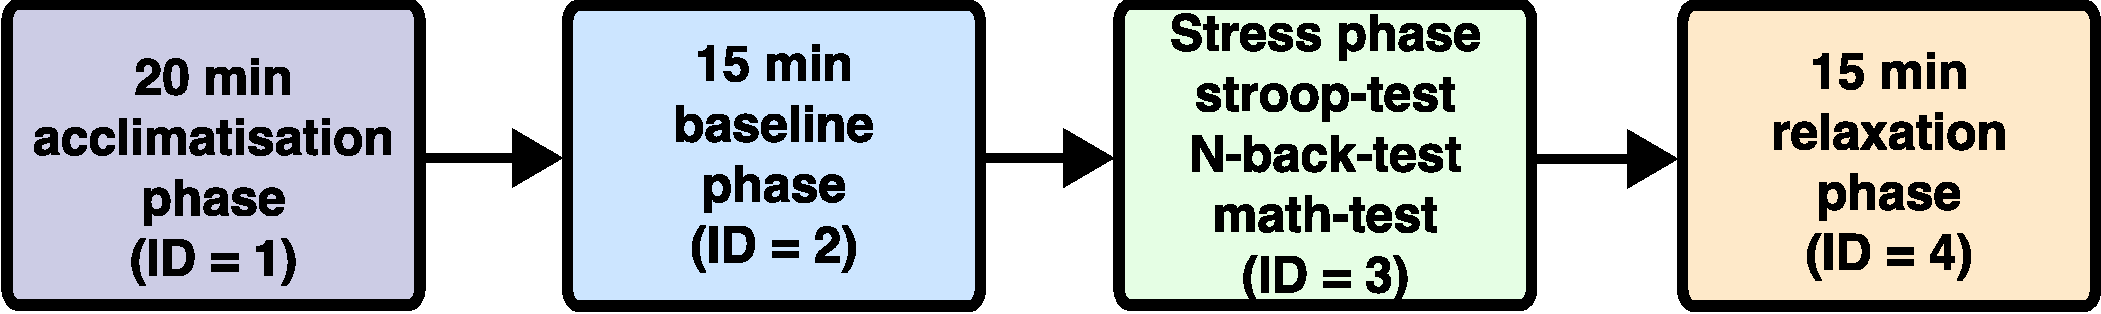
\includegraphics[width=0.95\linewidth]{../thesis-doc/images/study2/Procedure2_short.pdf}
\end{center}
\end{frame}

\begin{frame}
    \begin{center}
        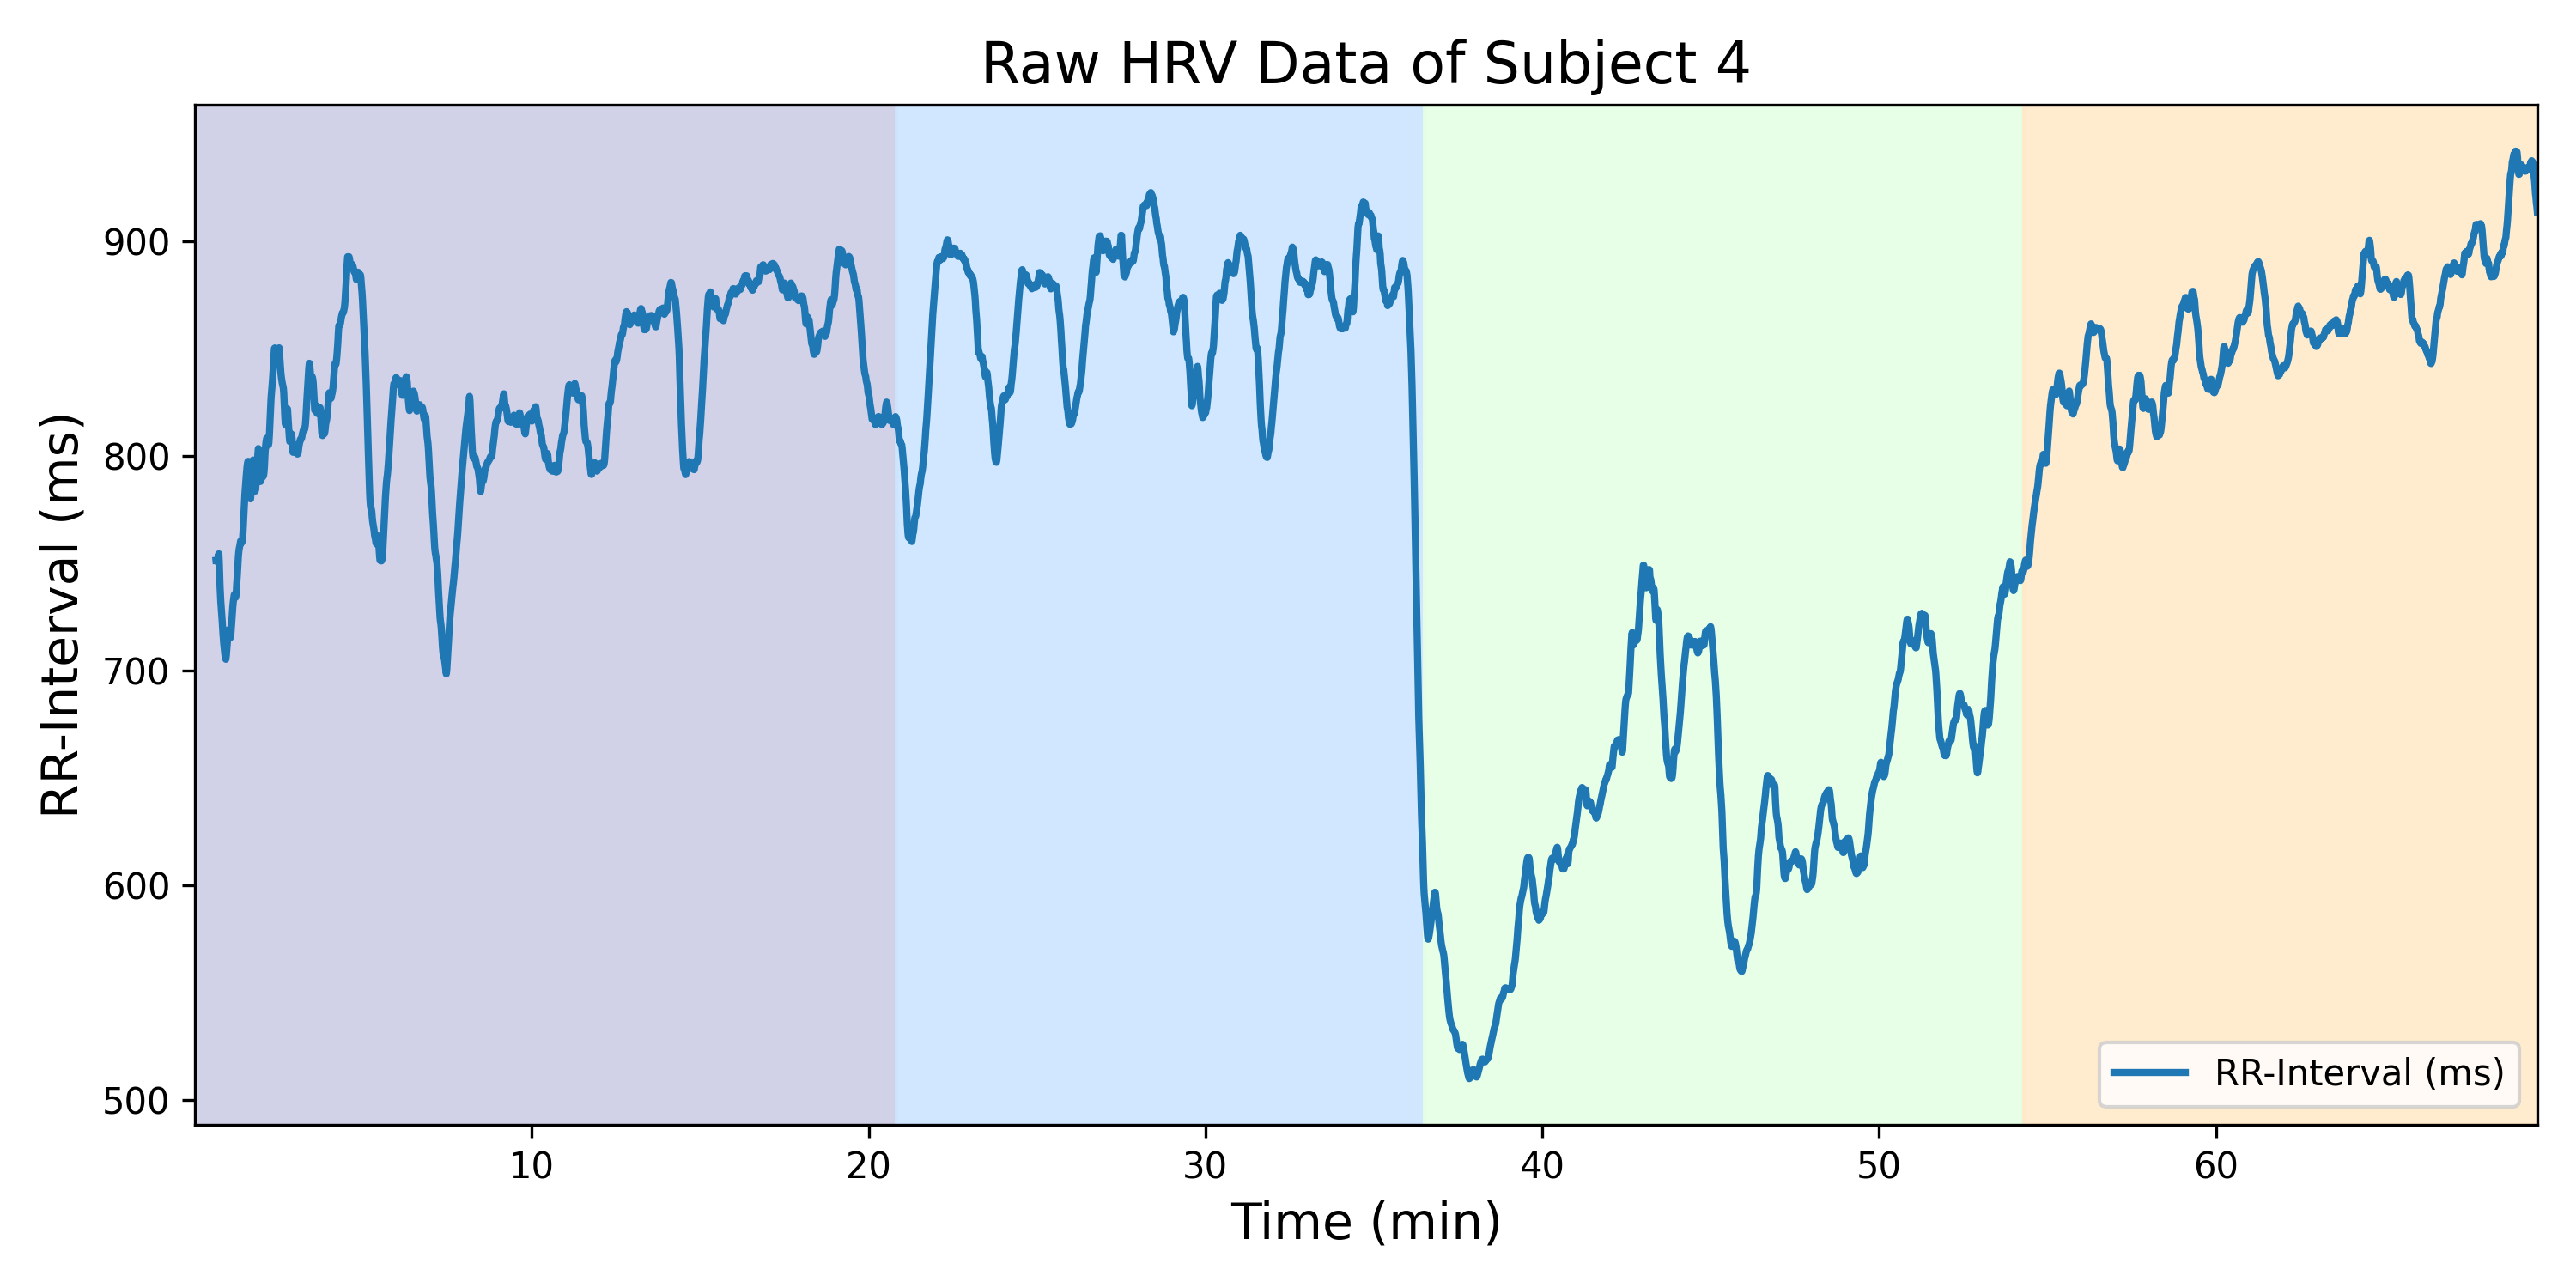
\includegraphics[width=0.9\linewidth]{../thesis-doc/images/study2/p04/raw_hrv_data_participant_4.png} 
    \end{center}
\end{frame}

\begin{frame}
    \begin{center}
        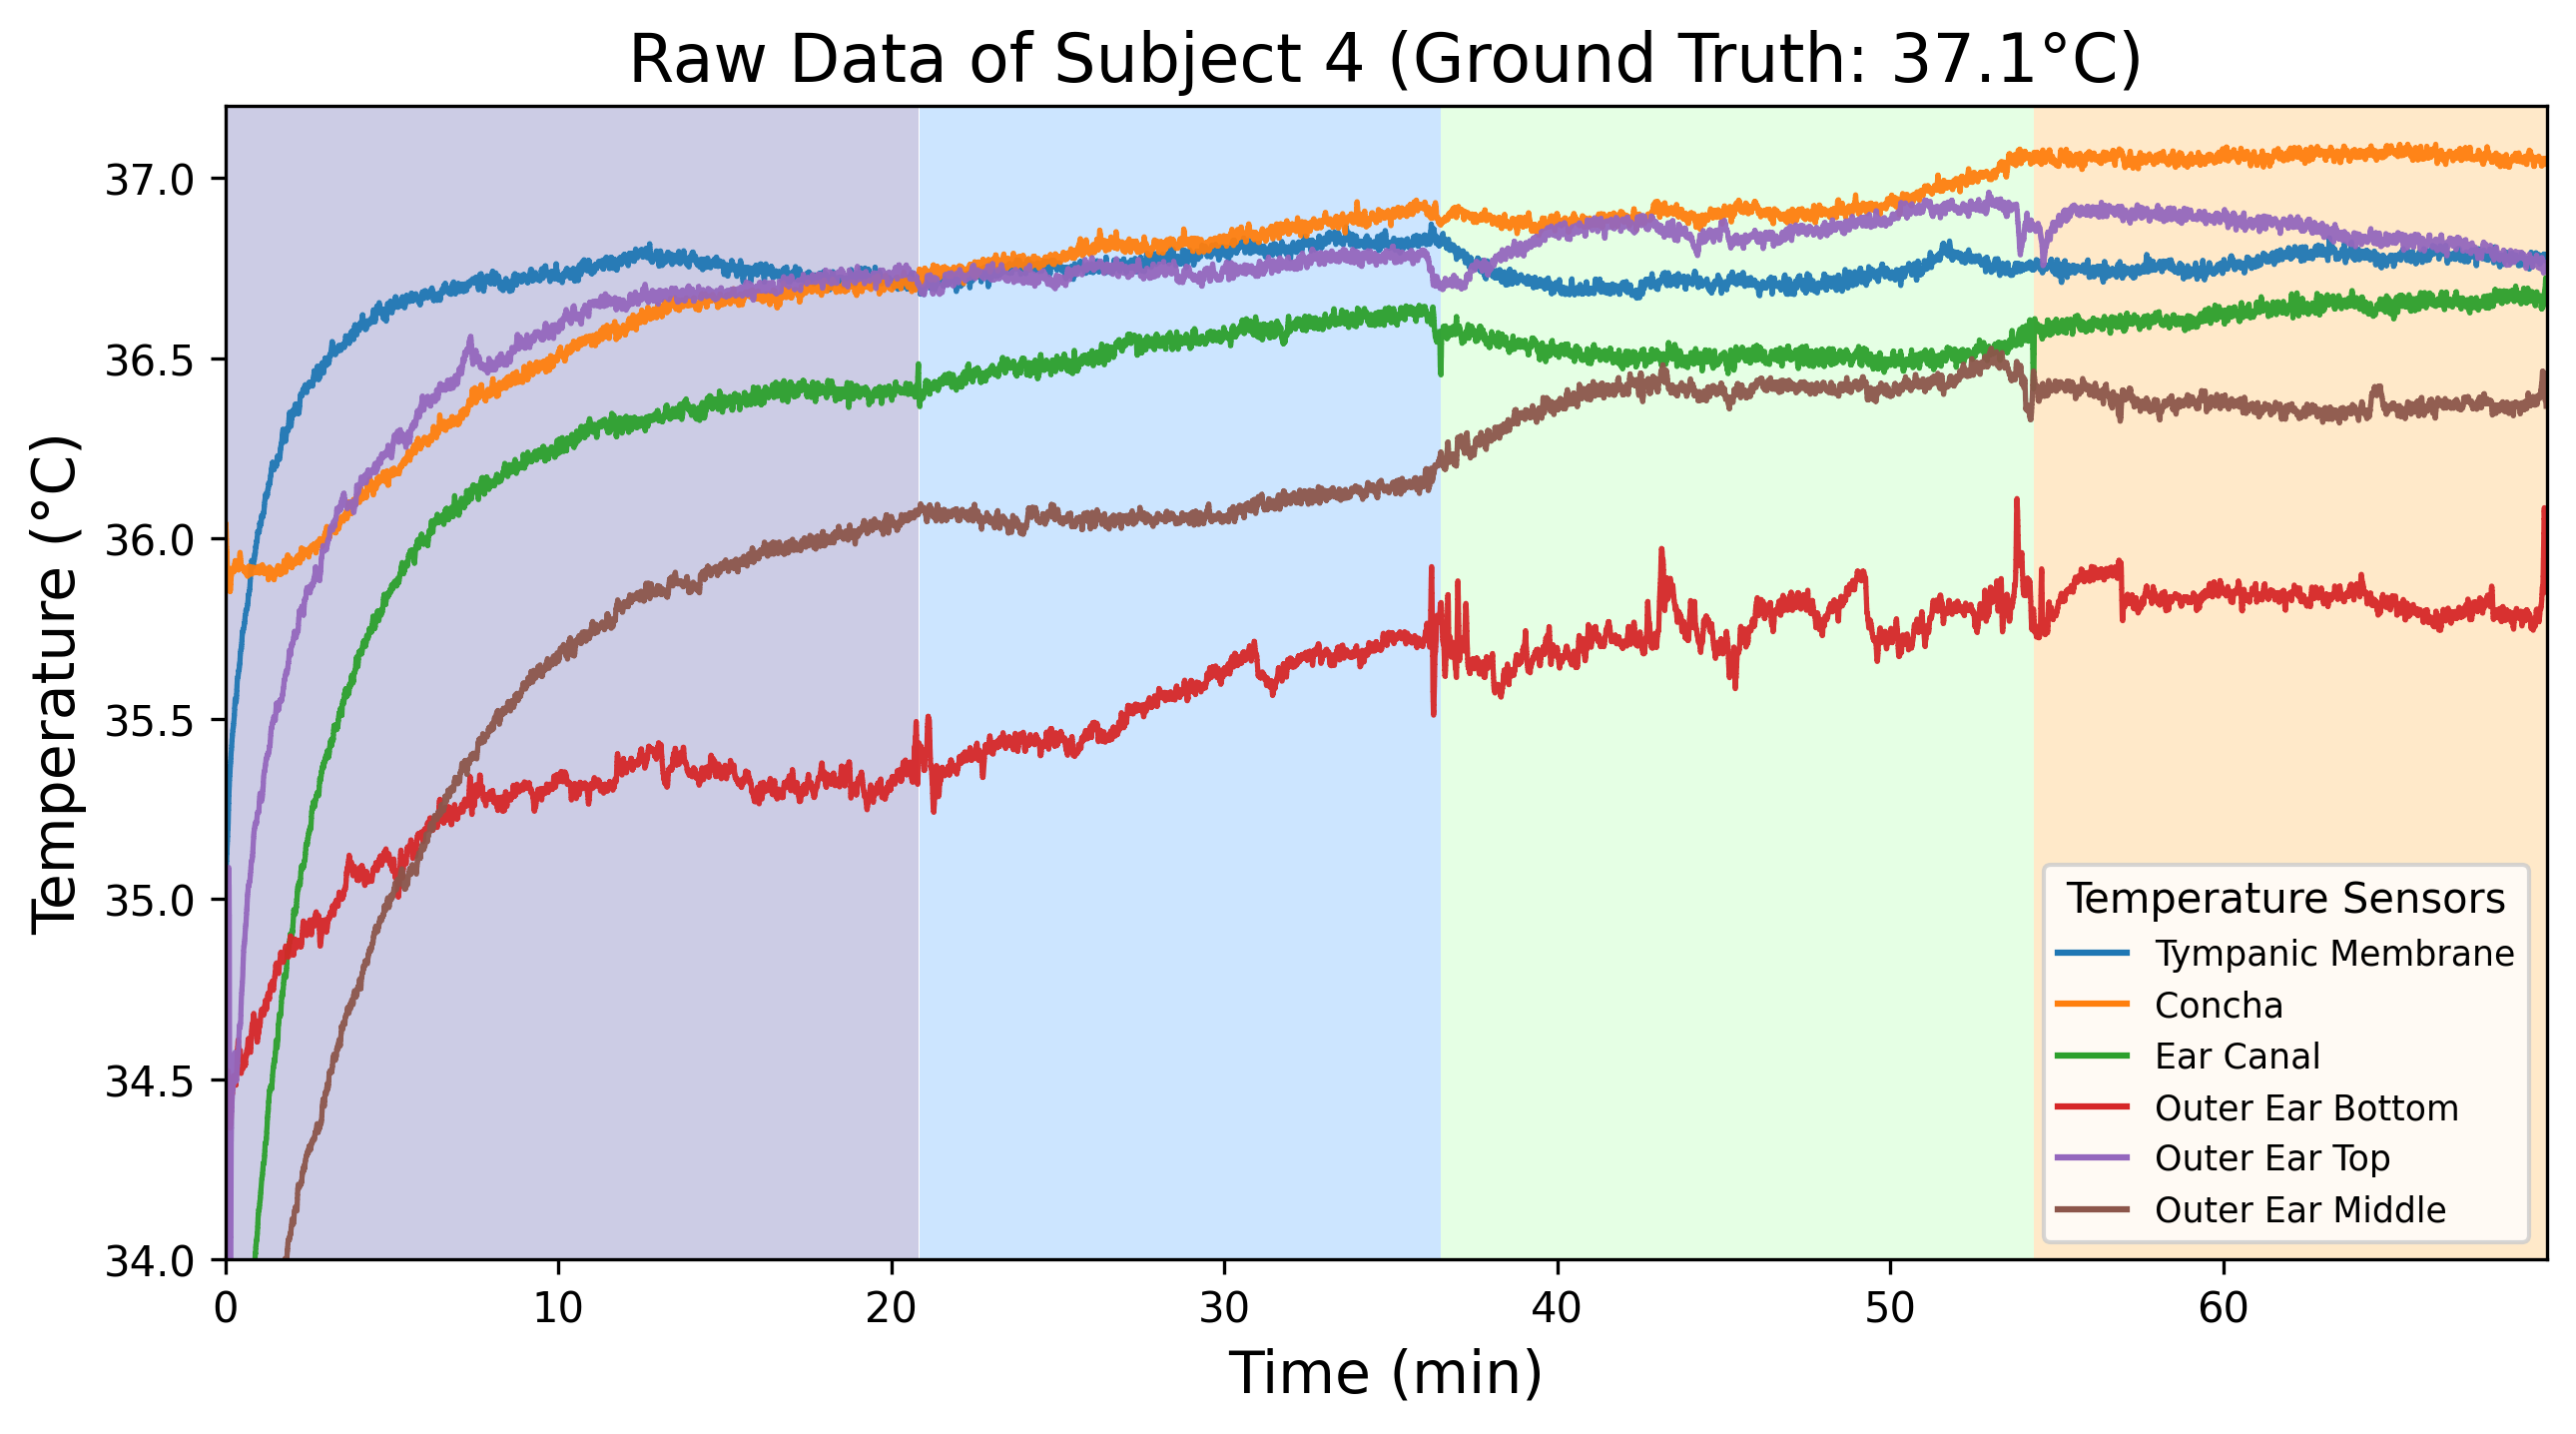
\includegraphics[width=0.9\linewidth]{../thesis-doc/images/study2/p04/Logging_study2_p04_0smoothed_raw_data.png} 
    \end{center}
\end{frame}

% \begin{frame}{Evaluation Study 2: Hypothesis 1}
%     \begin{itemize}
%         \item additional info or pictures
%     \end{itemize}
% \end{frame}

% \begin{frame}{Evaluation Study 2: Hypothesis 2}
%     \begin{itemize}
%         \item additional info or pictures
%     \end{itemize}
% \end{frame}

\section{Conclusion \& Future Work}
\begin{frame}{Conclusion}
    \begin{center}
      \begin{columns}[T]
        \begin{column}{.55\textwidth}
          \begin{itemize}
              \item Creation of a prototype
              \item 2 studies
              \begin{itemize}
                  \item Baseline and environmental influences
                  \item Under stress conditions
              \end{itemize}
              \item Findings:
              \begin{itemize}
                  \item Prototype for future studies
                  \item Long-term temperature monitoring while sitting/ sleeping
                  \item High potential to include motion data
              \end{itemize}
              
          \end{itemize}
        \end{column}
        
        \begin{column}{.4\textwidth}
          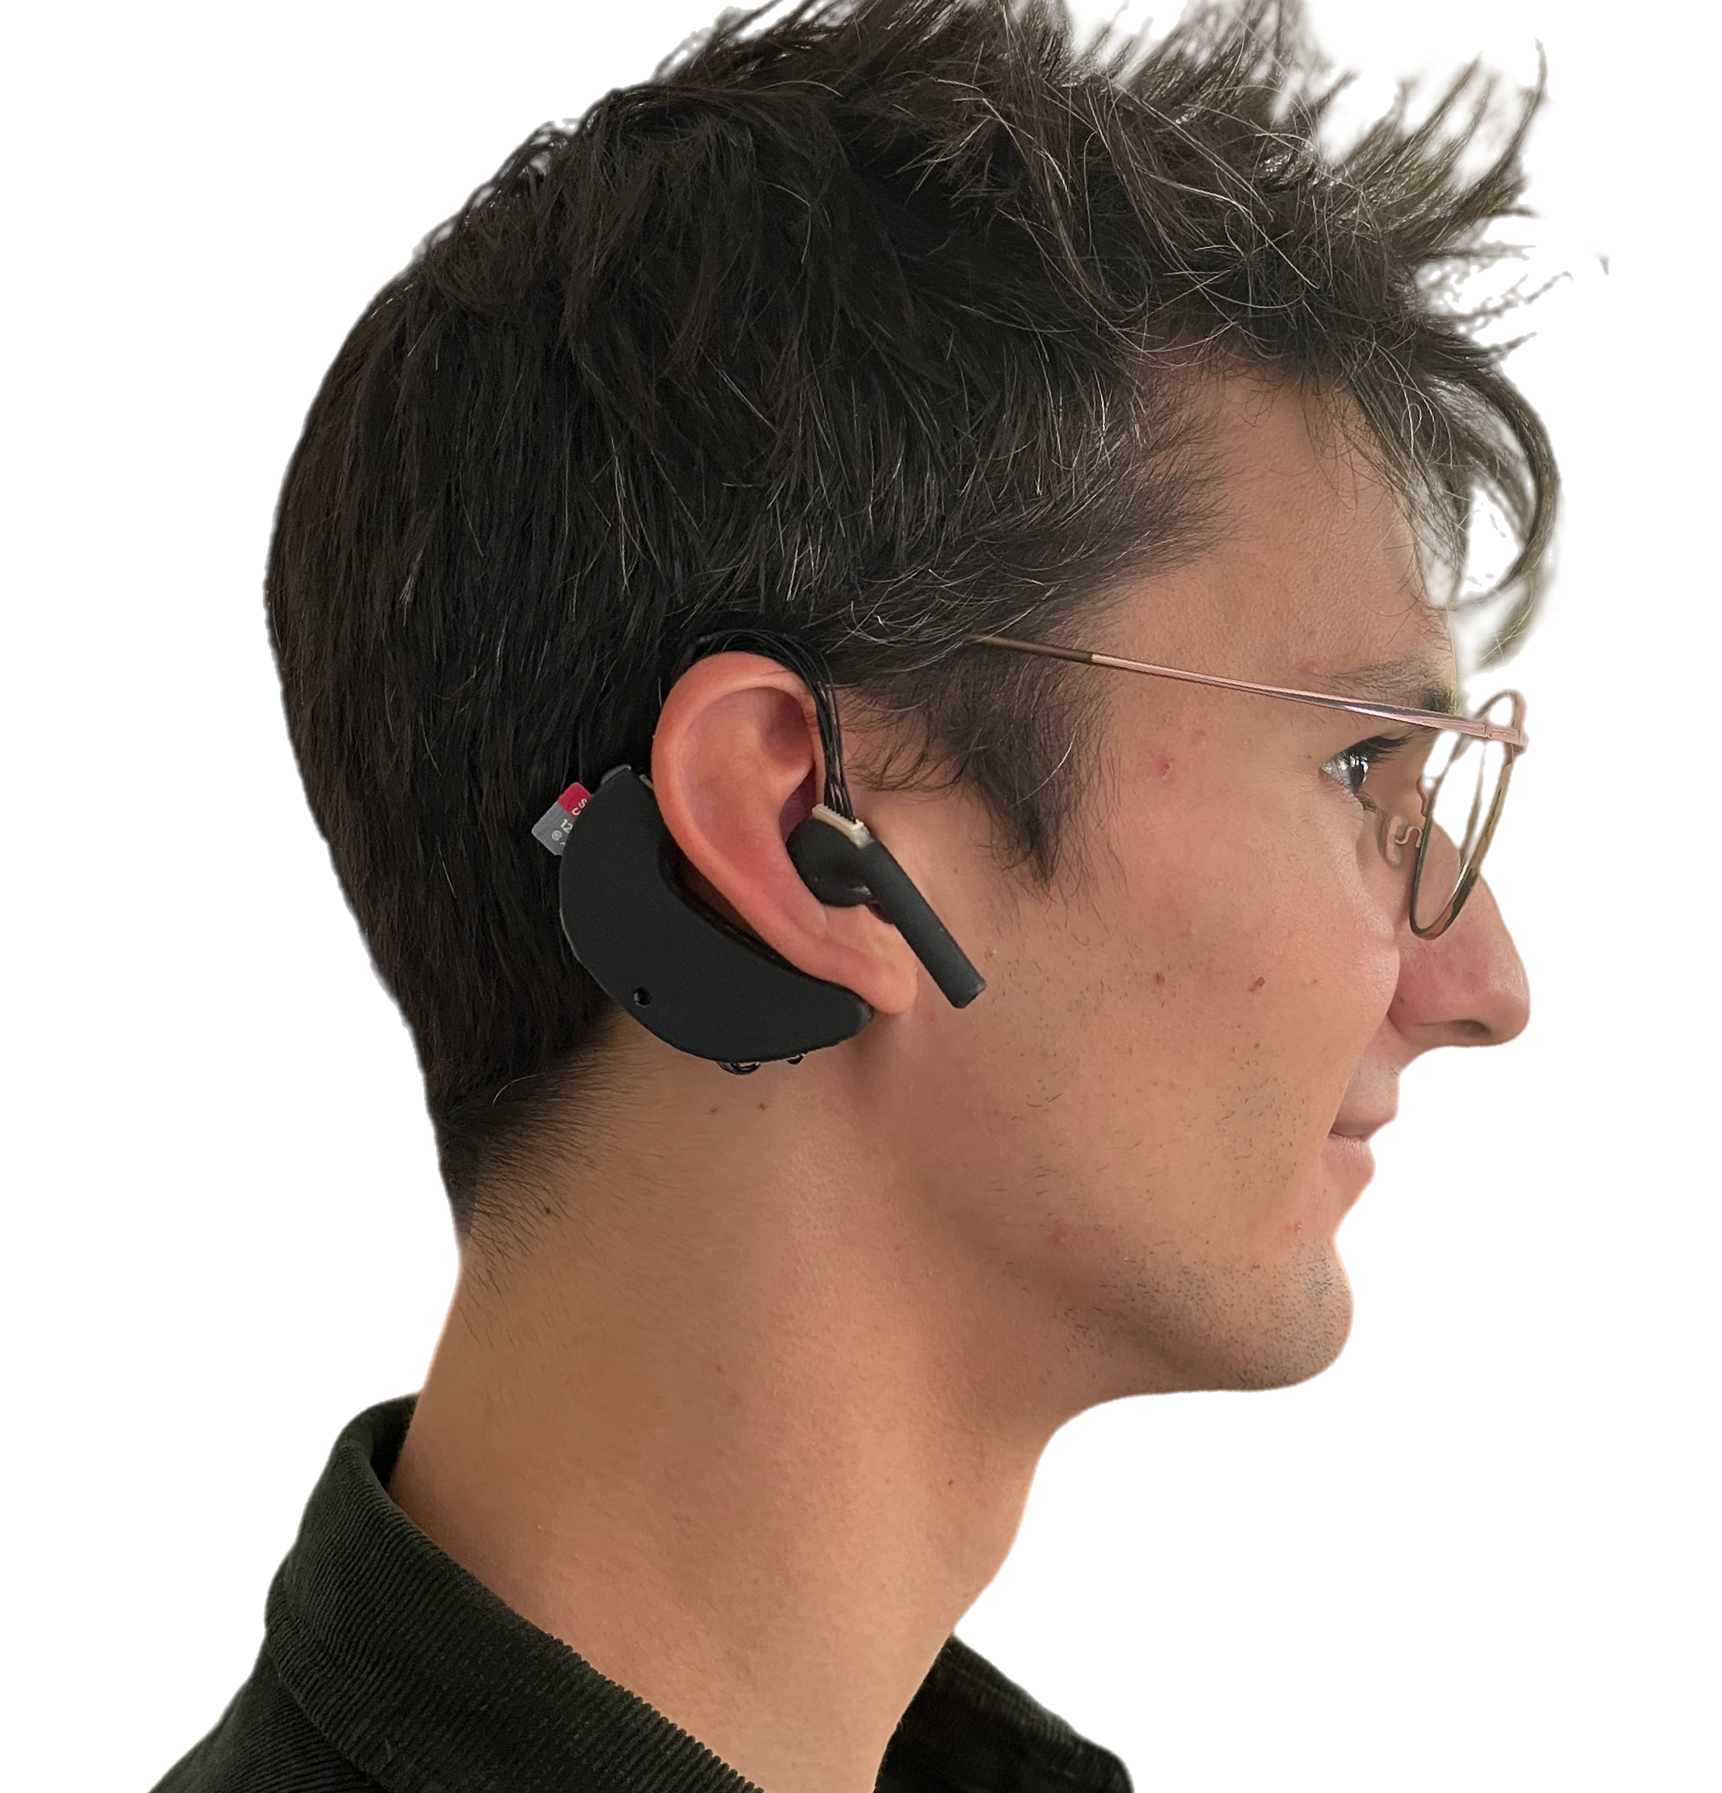
\includegraphics[width=0.8\linewidth]{../thesis-doc/images/prototype/Lorenz.png} 
        \end{column}
      \end{columns}
    \end{center}
\end{frame}

\begin{frame}{Future Work}
    \begin{itemize}
        \item TSST for Stress Detection with Increased Sample Size
        \item Detection of Circadian Rhythm
        \item Early Detection of Disease
        \item Cycle Tracking for Women
        % \item Real-World Applications
        % \item Approaches to Machine Learning
    \end{itemize}
\end{frame}

\appendix
\beginbackup


\begin{frame}{Literature}
    \printbibliography
\end{frame}

\section{Study Descriptions}
\begin{frame}
    \begin{center}
        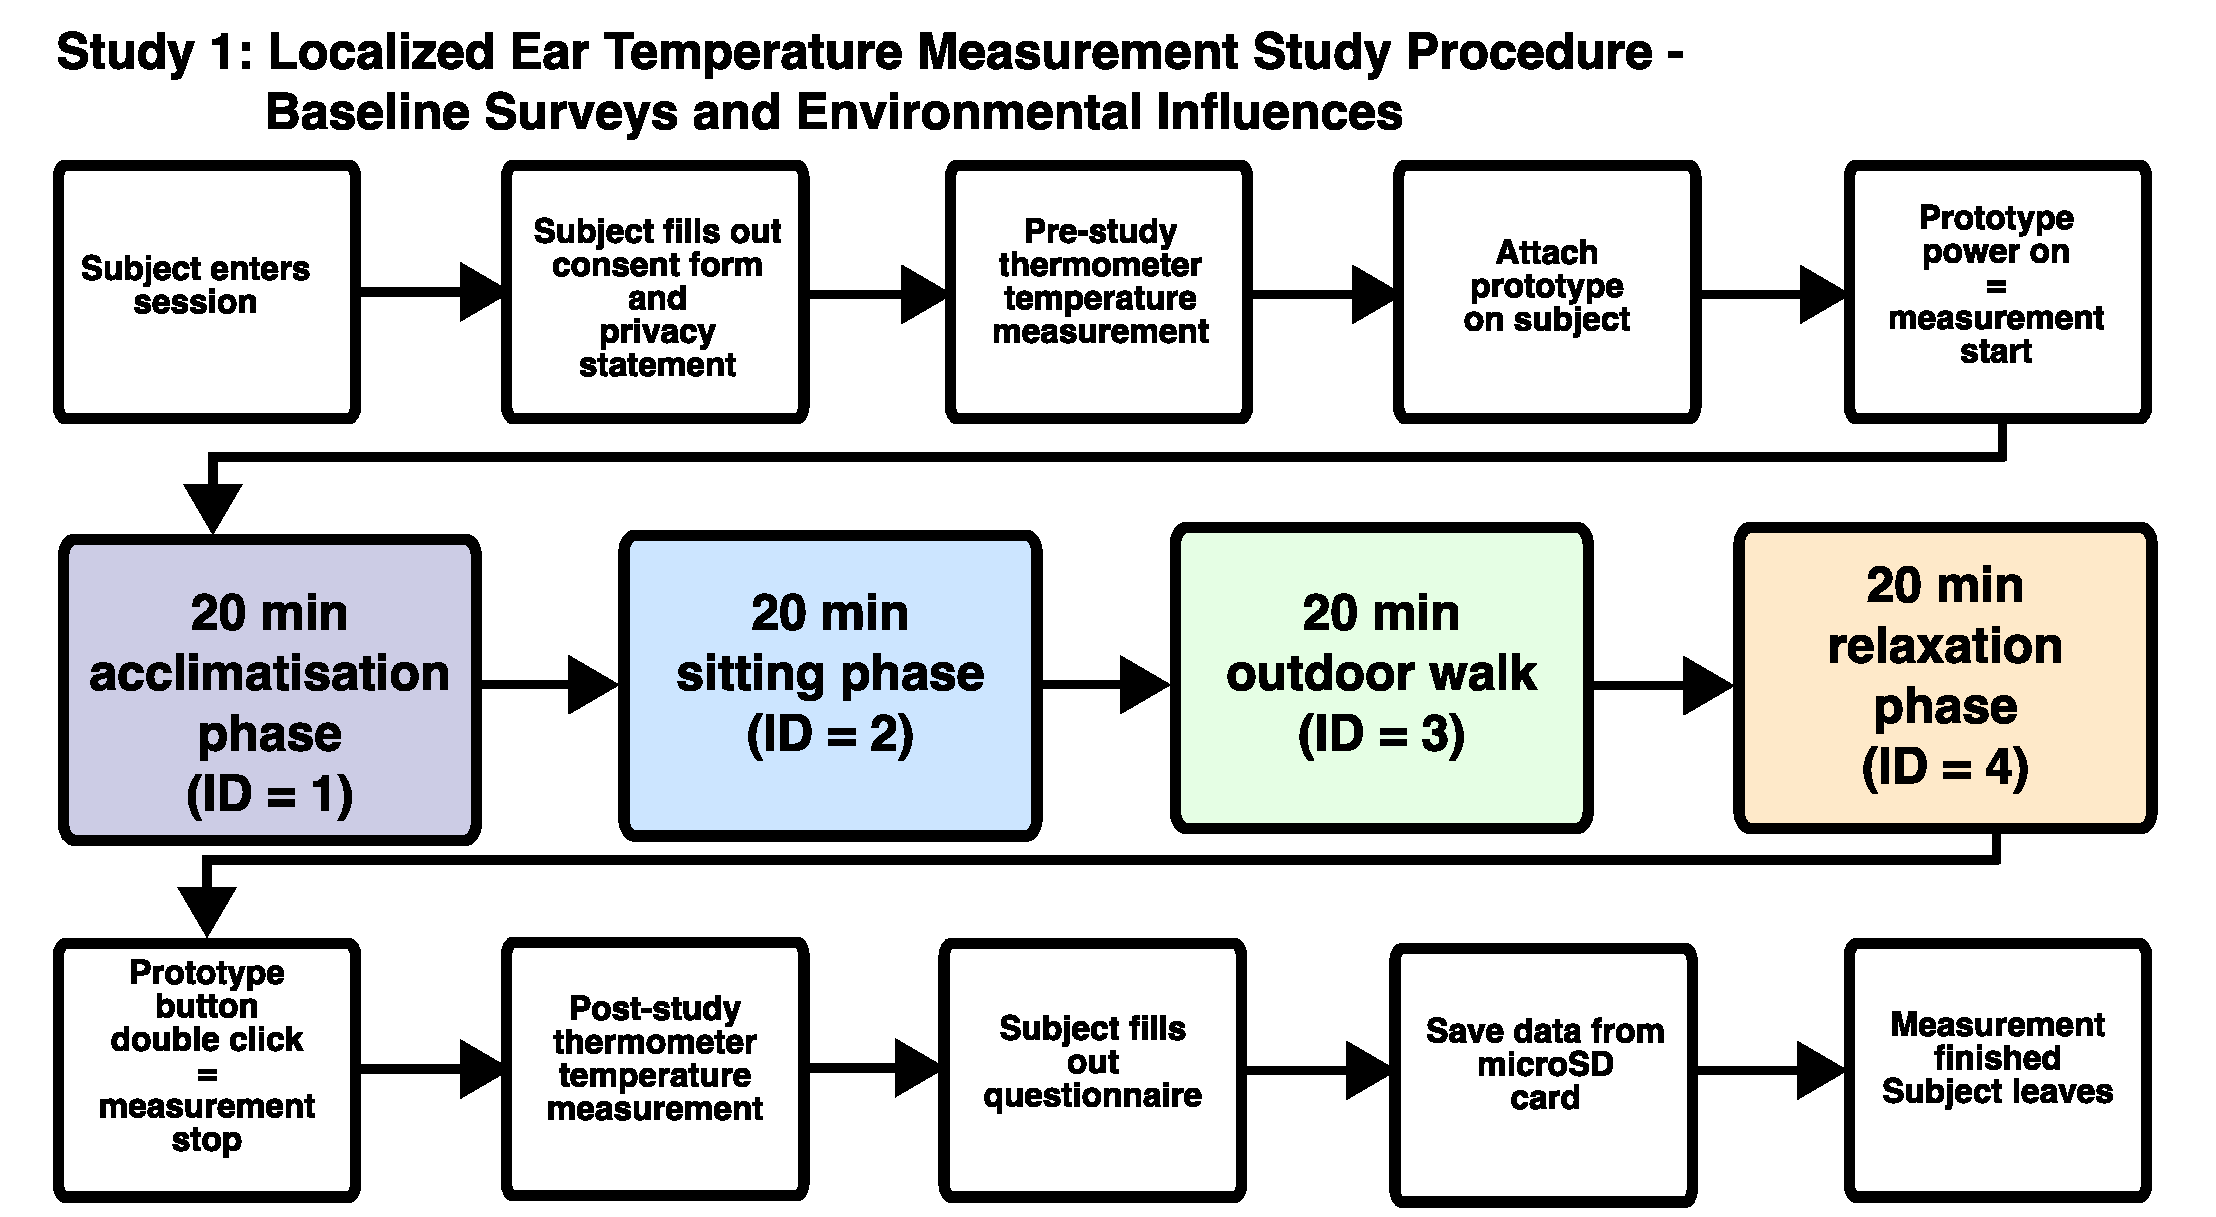
\includegraphics[width=0.9\linewidth]{../thesis-doc/images/study1/Procedure.pdf}
    \end{center}
\end{frame}

\begin{frame}
    \begin{center}
        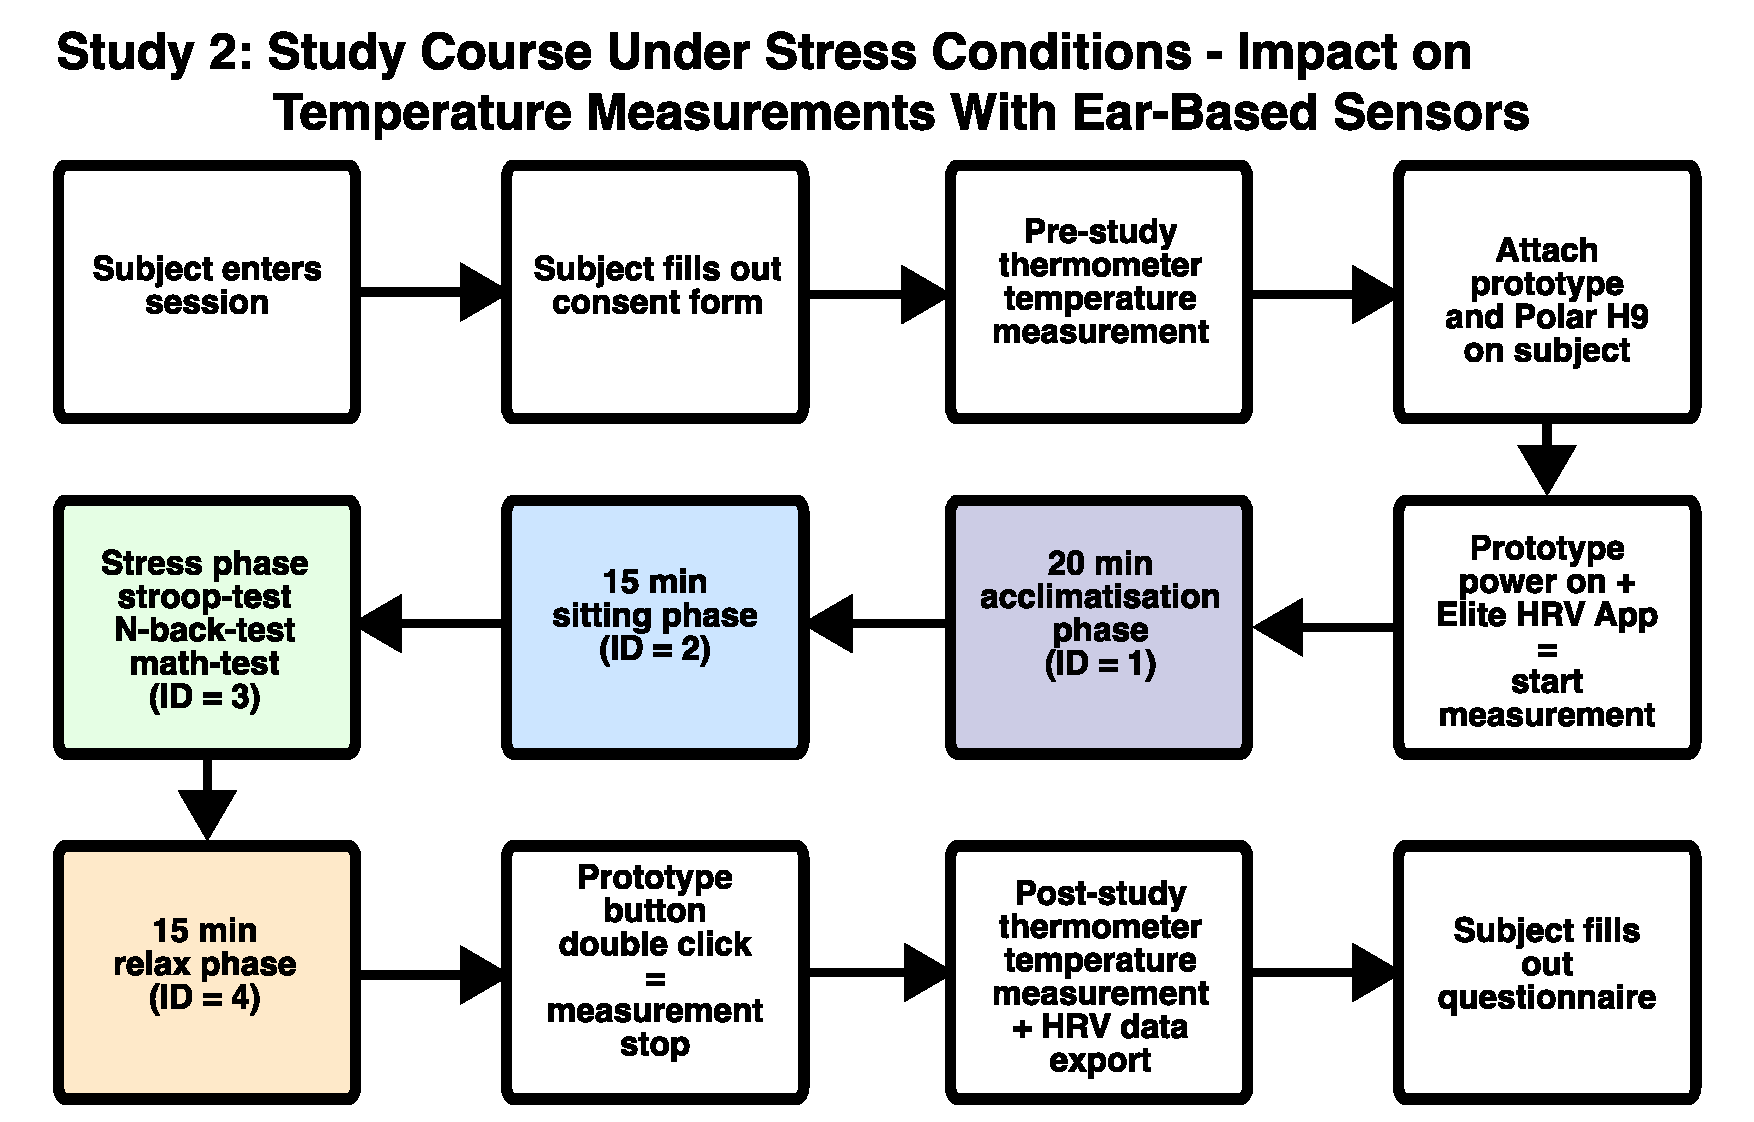
\includegraphics[width=0.9\linewidth]{../thesis-doc/images/study2/Procedure2.pdf}
    \end{center}
\end{frame}

\section{Implementation}
% \begin{frame}{Implementation}
%     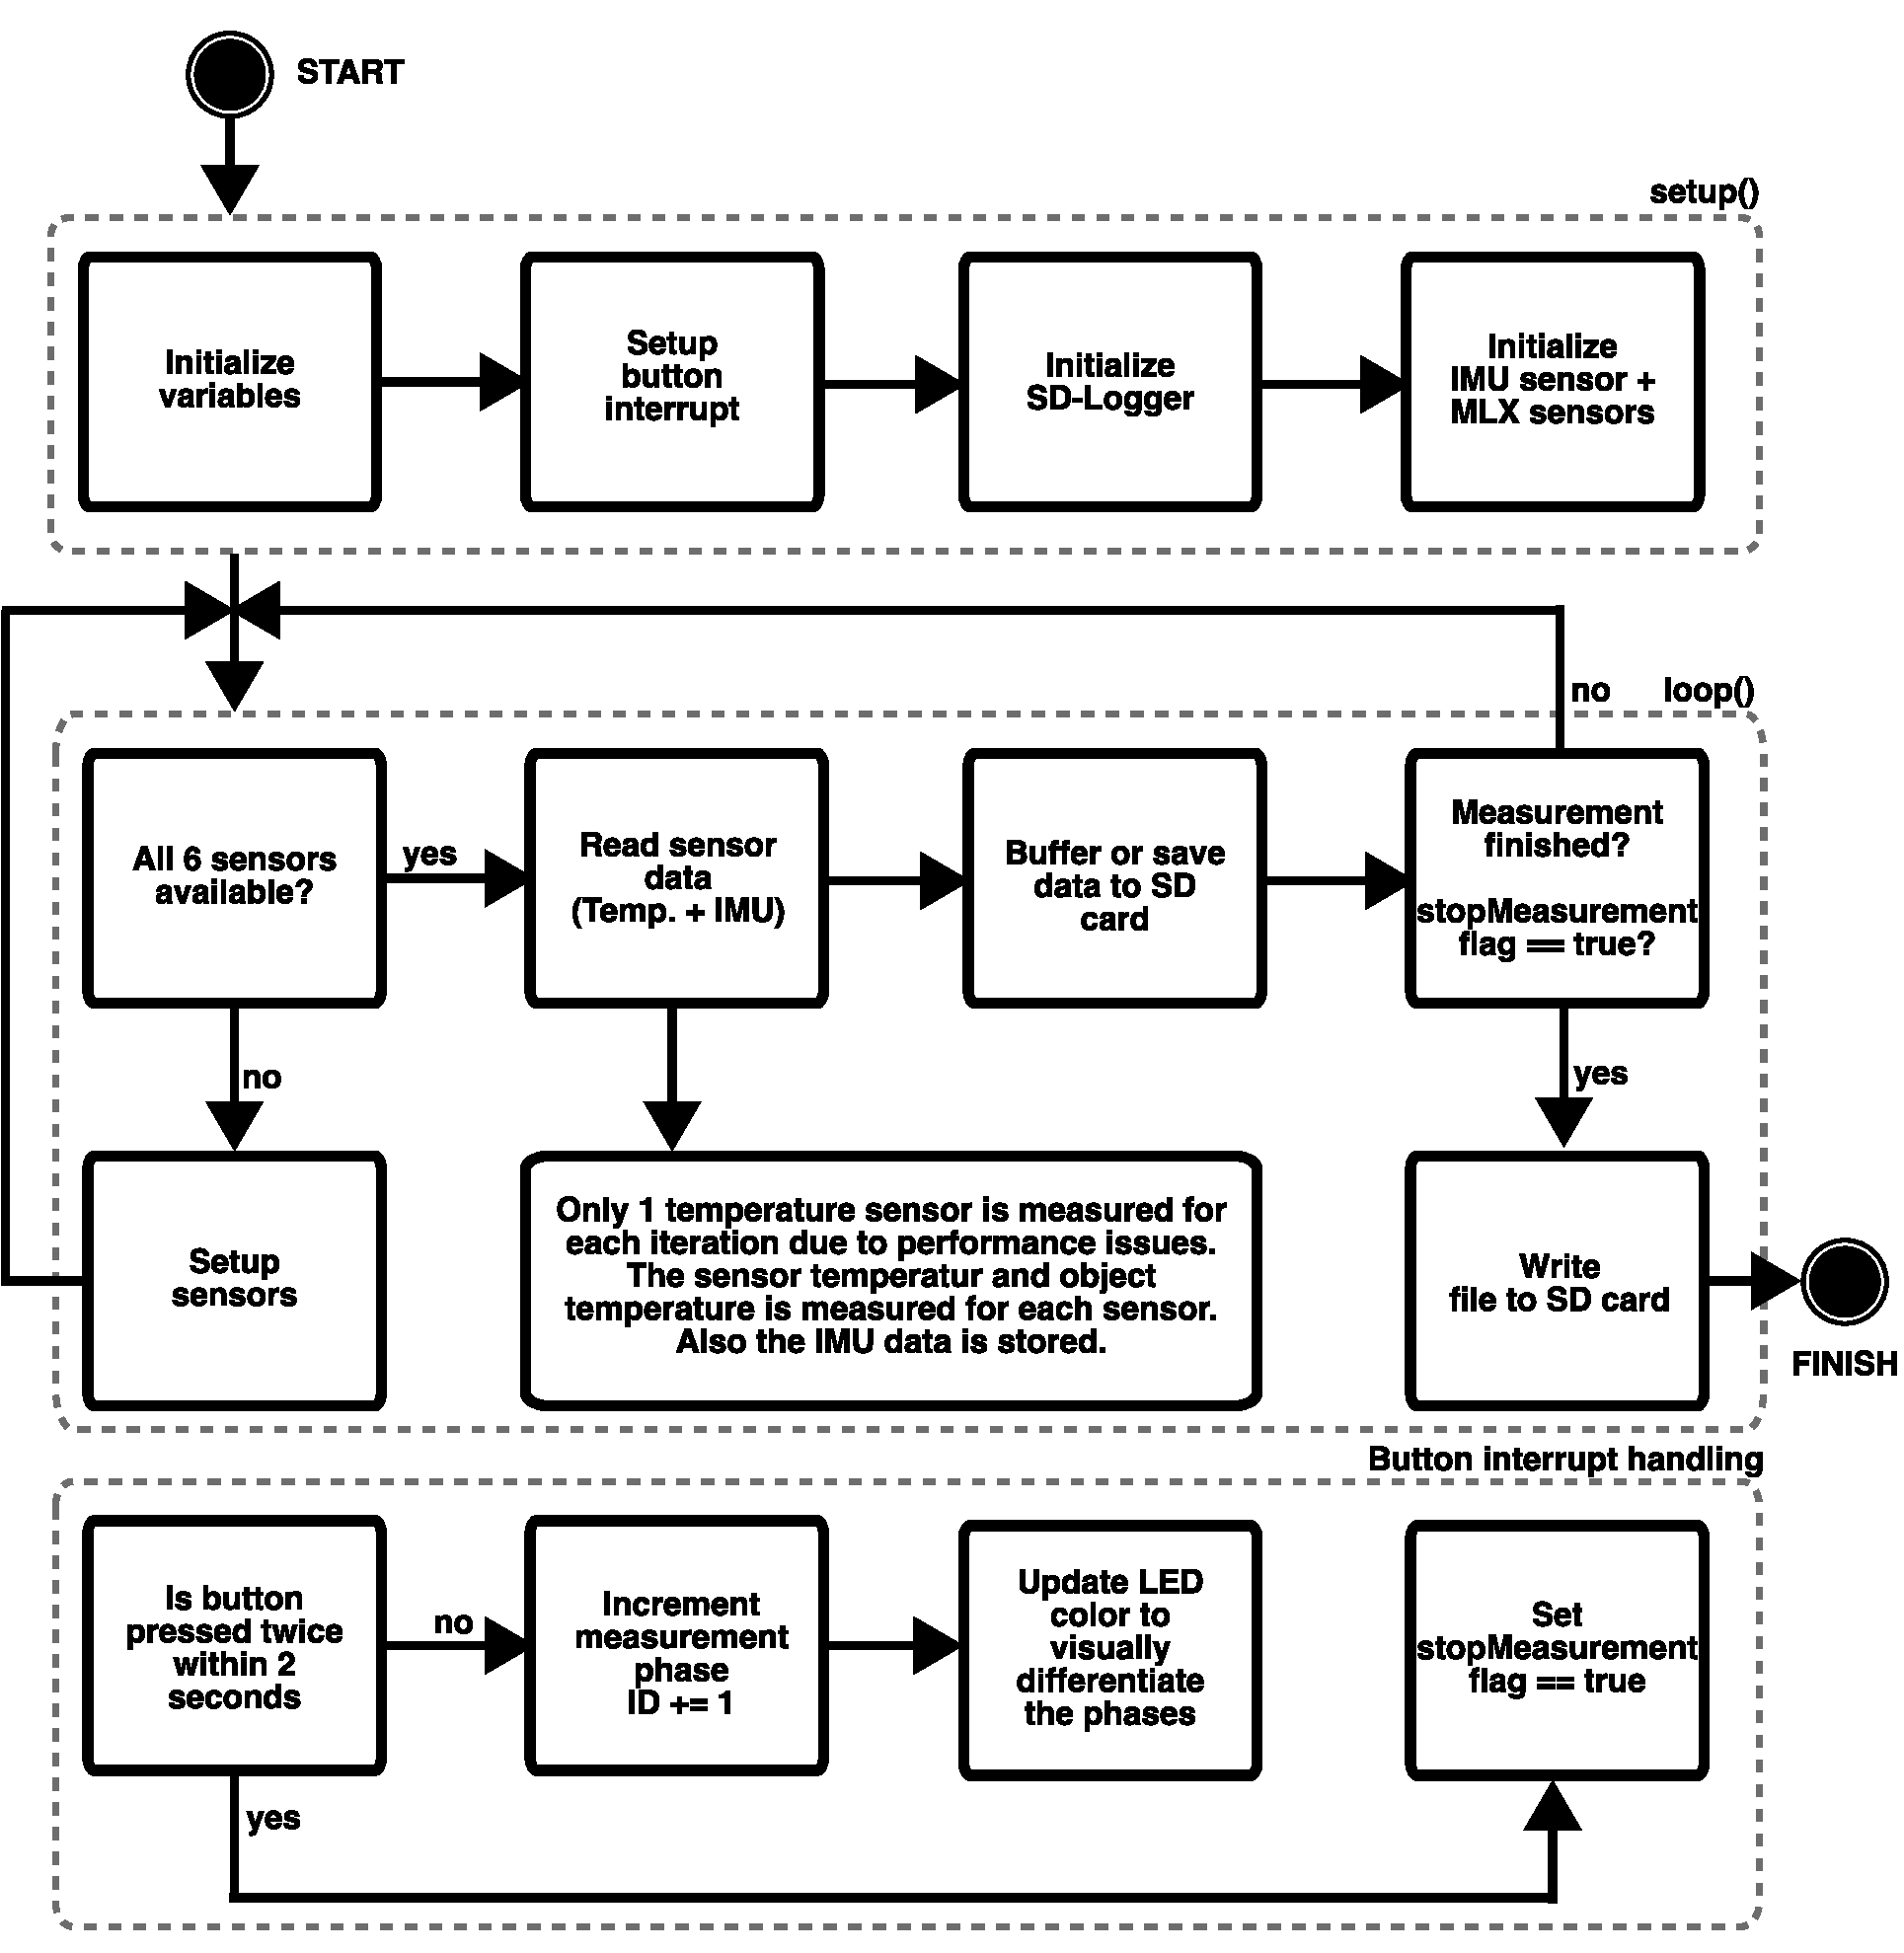
\includegraphics[width=0.45\linewidth]{../thesis-doc/images/ArduinoCodeProcedure.pdf}
% \end{frame}

\begin{frame}{Implementation}
    \begin{itemize}
        \item Arduino code
        \begin{itemize}
            \item setup() for initialization of temperature and IMU sensors and SD logger
            \item loop() for measuring data (temperature sensors with $8,3Hz$, imu data with $50Hz$)
        \end{itemize}
        \item Button action
        \begin{itemize}
            \item Single click: next phase
            \item Double click: stop measurement
        \end{itemize}
        \item Store data on SD-card
        \begin{itemize}
            \item 6 temperature sensors (object and sensor temperature)
            \item IMU data
            \item Timestamp
            \item ID (phase)
        \end{itemize}
    \end{itemize}
\end{frame}

\begin{frame}{Implementation}
    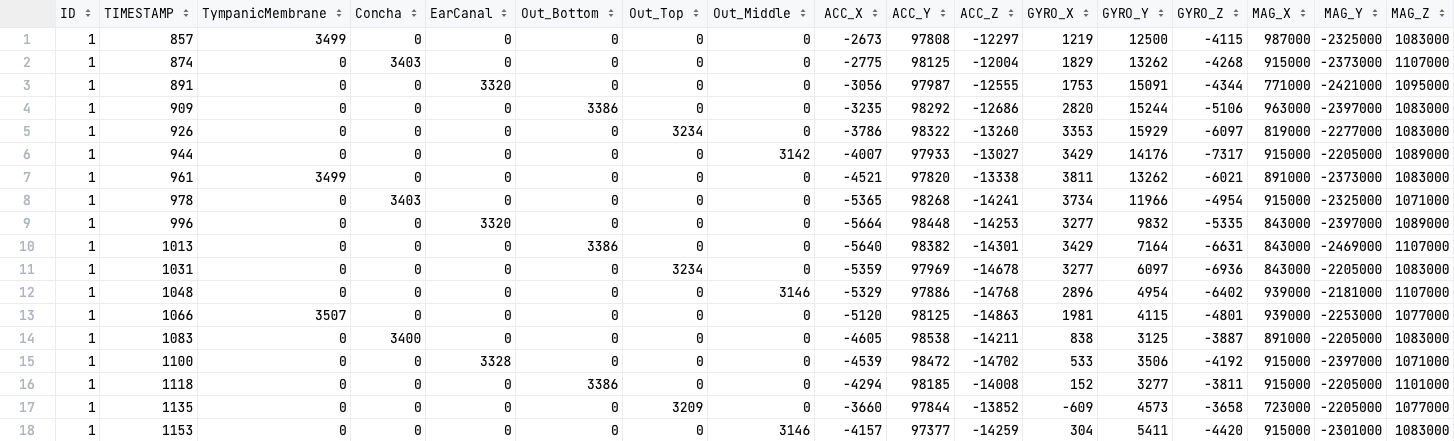
\includegraphics[width=\linewidth]{../thesis-doc/images/prototype/MeasurementRawDataSnippet_short.png}
\end{frame}

\backupend

\end{document}